\documentclass[12pt]{m-thesis}

\usepackage[dvipdfmx]{graphicx, color}
\usepackage{amsmath}
\usepackage{ascmac}
\usepackage{amsthm}
\usepackage{amssymb}
\usepackage{booktabs}
\usepackage{fancyvrb}
\usepackage{listings}
\usepackage{mediabb}
\usepackage{otf}
\usepackage{siunitx}
\usepackage{subcaption}
\usepackage{tabularx}
\usepackage{url}

\usepackage{algorithmic}
% \usepackage{algorithm}
\usepackage[ruled,vlined]{algorithm2e}

\lstset{
  backgroundcolor={\color[gray]{.90}},
  basicstyle={\ttfamily\small},
  breaklines=true,
  captionpos=b,
  frame=tRBl,
  keywordstyle={\ttfamily\small\bfseries},
  language=C,
  numbers=left,
  numberstyle={\ttfamily\small},
  showstringspaces=false,
  tabsize=2
}

% \makeatletter
% \def\lst@lettertrue{\let\lst@ifletter\iffalse}
% \makeatother

% \renewcommand{\lstlistingname}{コード}
% \renewcommand{\lstlistlistingname}{コード目次}

\begin{document}

\pagestyle{empty}

{\LARGE 修士論文} \hspace{\fill} {\LARGE 年度}
\begin{center}
  \vspace{5cm}
  {\huge 修論題目}\\
  \vspace{2cm}
  {\Huge 著者名}\\
  {\LARGE (学籍番号:)}\\
  \vspace{3cm}
  {\LARGE 指導教員 教授   寺岡 文男}\\
  {\LARGE 指導教員 専任講師 金子 晋丈}\\
  \vspace{2cm}
  {\Large 年3月}\\
  \vspace{1cm}
  {\LARGE 慶應義塾大学大学院理工学研究科}\\
  {\LARGE 開放環境科学専攻} \\
\end{center}

\clearpage
\newpage
\begin{center}
\Huge{論文要旨}
\end{center}

% Random Walk (RW) はグラフ解析技術として注目されている. 
% 一方, 解析対象となるグラフデータは近年大規模化が進み, WAN における転送コストの制約やプライバシ規制のため, 
% 一箇所に集中させず地理的に分散した環境下で保持されることが珍しくない. 
% しかしながら, このような WAN 環境では RTT やパケットロス率が増加するだけでなく, 
% グラフの全体把握が必要なグラフ分割も適用が困難となる. 
% 結果として主に単一データセンター内に保存されたグラフデータを対象とする既存 RW 手法を WAN 環境に適用すると
% 演算性能が大きく劣化する. 

% そこで本研究では, 地理的分散環境下であっても性能を維持することができる分散グラフ RW エンジンを提案する. 
% 提案手法は RW 演算の独立性に注目し, UDP を使用した非同期処理を採用した. 
% さらに Random Walker の経路再利用により通信量を削減する. 

% 地理的分散環境下を想定した実験の結果, 提案手法は既存手法に比べ $1.6 \sim 7.1$ 倍高速であることを明らかにした. 
% また提案手法は RTT, パケットロス率が大きくグラフ分割精度が悪いほど有効であり, 
% システム規模に対するスケーラビリティにも優れていることを明らかにした. 

Random Walk (RW) はグラフ解析技術として注目されている. 一方, 解析対象となるグラフデータは近年大規模化が進み, WAN における転送コストの制約やプライバシ規制のため, 一箇所に集中させず地理的に分散した環境下で保持されることが珍しくない. しかしながら, このような WAN 環境では RTT やパケットロス率が増加するだけでなく, グラフの全体把握が必要なグラフ分割も適用が困難となる. 結果として主に単一データセンター内に保存されたグラフデータを対象とする既存 RW 手法を WAN 環境に適用すると演算性能が大きく劣化する. 

そこで本研究では, 地理的分散環境下であっても性能を維持することができる分散グラフ RW エンジンを提案する. 提案手法は RW 演算が Random Walker (RWer) 単位で独立していることに注目し, UDP を使用した非同期処理を採用した. さらに RWer の経路再利用により RW 遷移時の通信量を削減する. 

地理的分散環境下を想定した実験の結果, 提案手法は既存手法に比べ $1.6 \sim 7.1$ 倍高速であることを明らかにした. また提案手法は RTT, パケットロス率が大きくグラフ分割精度が悪いほど有効であり, システム規模に対するスケーラビリティにも優れていることを明らかにした. 

\vspace{36pt}
\thispagestyle{empty}
\clearpage
\begin{center}
  \Huge{Thesis Abstract}\\
  \vspace{10pt}
  \large{}
\end{center}


Random Walk (RW) is widely used in graph analysis. The graph data to be analyzed are stored in data centers (DC) around the world, and it is necessary to analyze such globally distributed data for the operation of global search services. When analyzing such graphs, it would be desirable to collect all subgraphs in one centralized location and then analyze them, but this is not feasible due to the extremely high cost of communication over WANs caused by large graphs and graph changes, as well as privacy regulations. Therefore, it is important to develop a distributed graph RW execution engine in a geographically distributed environment. 
Considering that graphs will become larger and larger in the future, it is not realistic to execute RW from all vertices on a globally distributed graph, and it will become mainstream to execute RW starting from some vertices of interest. Therefore, in the execution of RW in the geographically distributed environment in this research, each DC is assumed to autonomously generate and process a Random Walker (RWer) starting from its own vertex, and the results are assumed to be utilized by the region where the DC is located. 
The existing distributed graph RW execution engine assumes execution in a single DC and performs synchronous processing using the Bulk synchronous parallel (BSP) model with TCP communication. However, under the geographically distributed environment assumed in this research, the performance of TCP communication in a low-bandwidth, high-latency WAN is greatly degraded, and the amount of communication for synchronization increases due to the increase of DCs. In addition, when the accuracy of graph partitioning as a whole is deteriorated by editing the graph for each DC, the number of synchronization cycles among DCs increases due to the increase of RW transitions among DCs. Therefore, this existing method is not suitable for the environment envisioned in this research.
In this paper, we propose a distributed graph RW execution engine suitable for geographically distributed environments. The proposed method employs asynchronous processing using UDP communication, by paying attention to features of RW operations such as independence per RWer and being aware of the application of the proposed method. By using UDP communication, the performance degradation in WAN can be suppressed. And asynchronous processing eliminates the need for costly synchronous communication and enables autonomous RW execution by each data center. Moreover, the proposed method can skip some RWer transmissions during RW transitions by reusing the routes of RWers that have been terminated in the past.
Experimental results in a geographically distributed environment show that the proposed method is 1.6 (without route reuse) ~ 7.1 (with route reuse) times faster than the existing methods. Unlike existing methods, the proposed method is effective when the RTT, and packet loss rate are large and the accuracy of graph partitioning is poor. The proposed method is also found to have excellent scalability with respect to the system size. This is because the performance of the proposed method does not deteriorate when the number of servers is increased.

\vspace{36pt}
\thispagestyle{empty}
\clearpage
\typeout{Indexes}
\setcounter{page}{1}
\pagenumbering{roman}
\tableofcontents
\thispagestyle{plain}
\listoffigures
\listoftables
% \lstlistoflistings
\clearpage

\pagestyle{headings}
\setcounter{page}{1}
\pagenumbering{arabic}

\chapter{序論}
\label{chap:intro}
\section{背景}

Random Walk (RW) は図 \ref{Random Walk の概要} に示すように, グラフ上で Random Walker (RWer) が確率 $\alpha$ で終了し, 確率 $1 - \alpha$ でランダムな隣接頂点に遷移するアルゴリズムであり, グラフ解析において広く利用されている. RW を用いたグラフ演算の例として, Personalized PageRank \cite{PPR} (PPR) がある. PPR により, ある頂点から見た他の頂点の関連度を算出することができる. 例えば Web ページを頂点, Webページ間の参照関係をエッジとしたグラフ上で PPR 演算をすることで, Web サイトの推薦システムを作成することができる. 他にも RW は, コミュニティ検出, リンク予測, 類似性推定や機械学習等のアプリケーションで利用される. 

% 解析対象となるデータは世界中で日々増加し, 各地域のデータセンターに保存される. 例えば, Amazon Web Service は全世界の 33 箇所の地域にそれぞれクラウドインフラストラクチャを保有している \cite{aws} . 世界規模で展開されるサービスの運用のためには, 世界中に分散したデータを解析する必要がある. 図 \ref{地理的分散環境下におけるグラフ} に地理的分散環境下でのグラフ管理のイメージを示す. データセンター 1, 2, 3 が各々部分グラフを管理しており, 一部頂点は異なるデータセンターが保持する頂点へのエッジを持つ. このようなグラフを解析するとき, 中央集権的に全ての部分グラフを一箇所に集めてから解析することが理想だが, 以降に述べる理由によりこれはコストが非常に高い, もしくは実現不可能である. まずグラフの規模が非常に大きく, グラフの変化も頻繁に発生するため, 広域ネットワーク (WAN) での転送コストが高い. また, GDPR のようなプライバシー規制によって, その地域のデータセンターに保存されている元データを転送できない場合も考えられる. そのため, 地理的に分散した環境下におけるグラフ解析 (本研究では RW) のためのシステム開発が重要となる. 

解析対象となるデータは世界中で日々増加し, 各地域のデータセンターに保存される. 例えば, Amazon Web Service は全世界の 33 箇所の地域にそれぞれクラウドインフラストラクチャを保有している \cite{aws} . 世界規模で展開される検索サービスの運用のためには, 世界中に分散したデータを解析する必要がある. 中でもグラフにおけるデータ解析は, PageRank Web 検索\cite{334}, SNS 検索\cite{10.5555/2535461.2535468}, ナレッジグラフ検索\cite{10.1145/3331184.3331252} など, 多くの一般的なインターネットサービスの基盤となっている.  
% 中でも RW によるグラフ解析は PPR, グラフ推定など, 比較的グラフ内の局所的なデータ解析に用いられることが多い. 

世界中に分散した解析対象グラフは現状で数十億頂点, 数兆エッジと巨大であり, 将来はさらに巨大化していくと予想する. このようなグラフを解析するとき, 中央集権的に全ての部分グラフを一箇所に集めてから解析することが理想だが, 以降に述べる理由によりこれはコストが非常に高い, もしくは実現不可能である. まずグラフの規模が非常に大きく, グラフの変化も頻繁に発生するため, 広域ネットワーク (WAN) での転送コストが高い. また, GDPR のようなプライバシー規制によって, その地域のデータセンターに保存されている元データを転送できない場合も考えられる. そのため, 地理的に分散した環境下におけるグラフ解析 (本研究では RW) のためのシステム開発が重要となる. 

地理的分散環境下における RW はグラフ内の局所的なデータ解析に用いられることが多いと考える. これは, 今後グラフがより大規模化していくことを考慮すると, 全世界に分散するグラフ上の全頂点から RW を実行することは現実的ではなく, 興味がある一部頂点を始点とした RW の実行が主流になるからである. そしてこの RW 実行は各地域(データセンター)ごとに独立して行われる. つまり, 各データセンターが, 自身が保有する頂点を始点とした RWer の生成・ 処理を自律的に行い, その RW 結果をそのデータセンターの所在地域が活用することとなる. 

既存の分散グラフ RW 実行エンジン \cite{10.1145/3341301.3359634} は単一のデータセンター内での実行を想定しており, 地理的分散環境下のような RTT, パケットロス率が高い環境では大きく性能が劣化することが本研究の評価からも示されている. この手法ではサーバ間での RWer 送受信に TCP 通信を採用しており, 地理的分散環境下ではスループットが小さくなるためである. また, 既存手法は Bulk synchronous parallel (BSP) モデルによる同期処理を行うが, この処理方式は本研究が想定する地理的分散環境下における自律的な RW 実行には適さないと考える. まず, 同期処理をする場合サーバ間同期のための通信 (RWer 遷移のための通信) が何度も発生するが, WAN のような低帯域・高遅延の環境ではこの通信のオーバヘッドが増加する. これはシステムのスケーラビリティにも悪い影響を与える. また, データセンターごとのグラフ編集により全体として見たときのグラフ分割精度が悪くなってしまう場合, データセンター間を跨ぐエッジが増加し同期の回数が増えるため, 性能が悪化する. 
% さらに, 各データセンターによる自律的な RW 実行という要件に反する. 

そこで本研究では, 地理的分散環境下に適した分散グラフ RW 実行エンジンを提案する. 提案手法は, 本手法の用途を意識することに加え, RWer 単位での独立性という RW 演算の特徴に注目し, UDP 通信を使用した非同期処理を採用した. UDP 通信を利用することで, WAN におけるスループットの低下を抑えられる. そして非同期処理を採用することで高コストな同期通信を省略し, 各データセンターによる自律的な RW 実行を実現することができる. また, 提案手法は過去に終了した RWer の経路を再利用することで, RW 遷移時の通信量を削減する機能を有する. 地理的分散環境下を想定した実験によって, 提案手法が既存手法よりも実行時間やグラフ分割精度変化に対する耐性, システム規模に対するスケーラビリティの観点で適切な手法であることを明らかにする. 

\begin{figure}[t]
    \centering
    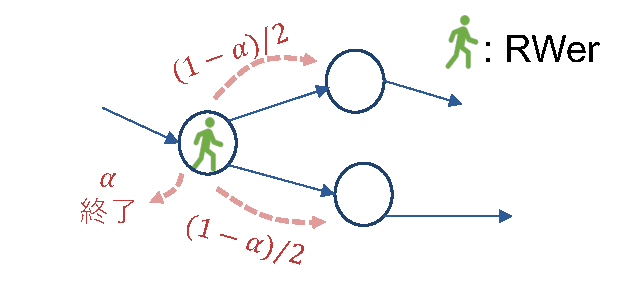
\includegraphics[scale=1.0]{figure/RandomWalk.pdf}
    \caption{Random Walk の概要.}
    \label{Random Walk の概要}
\end{figure}

\section{地理的分散環境下におけるグラフの定義}

図 \ref{地理的分散環境下におけるグラフ} に本研究が想定する地理的分散環境下でのグラフ管理の概要を示す. データセンター (DC) 1, 2, 3 が各々部分グラフを管理しており, 一部頂点は異なる DC が保持する頂点へのエッジを持つ. つまり各 DC は自分が保持する頂点の隣接頂点のうち, 他の DC が保有する頂点の情報 (頂点 ID, 持ち主 DC ) も持つ. ただしこの他 DC の頂点の隣接頂点情報は保持しない. 例えば図 \ref{地理的分散環境下におけるグラフ} において,  DC  1 は自分が保持する頂点 4 の隣接頂点である頂点 10 の情報 (頂点 ID = 10, 持ち主 DC  =  DC  2), を持つが, 頂点 10 が頂点 7 や頂点 8 と隣接していることは知らない. 

% DC 間における通信環境は WAN であり, RTT, パケットロス率が高い. また, 各 DC が独立してグラフの編集を行うため, 全体として見たときの各 DC によるグラフ分割精度は制御不能である.  
DC は地理的に離れた位置に設置されており, DC 間の RTT, パケットロス率が高くなる. 現実世界では各 DC は数十億頂点の部分グラフを所持しており, DC 間を跨ぐエッジは数十億エッジ $\sim$ 数兆エッジと想定する. また, 各 DC が独立してグラフの編集を行うため, 全体として見たときの各 DC によるグラフ分割精度は制御不能である.

\begin{figure}[t]
    \centering
    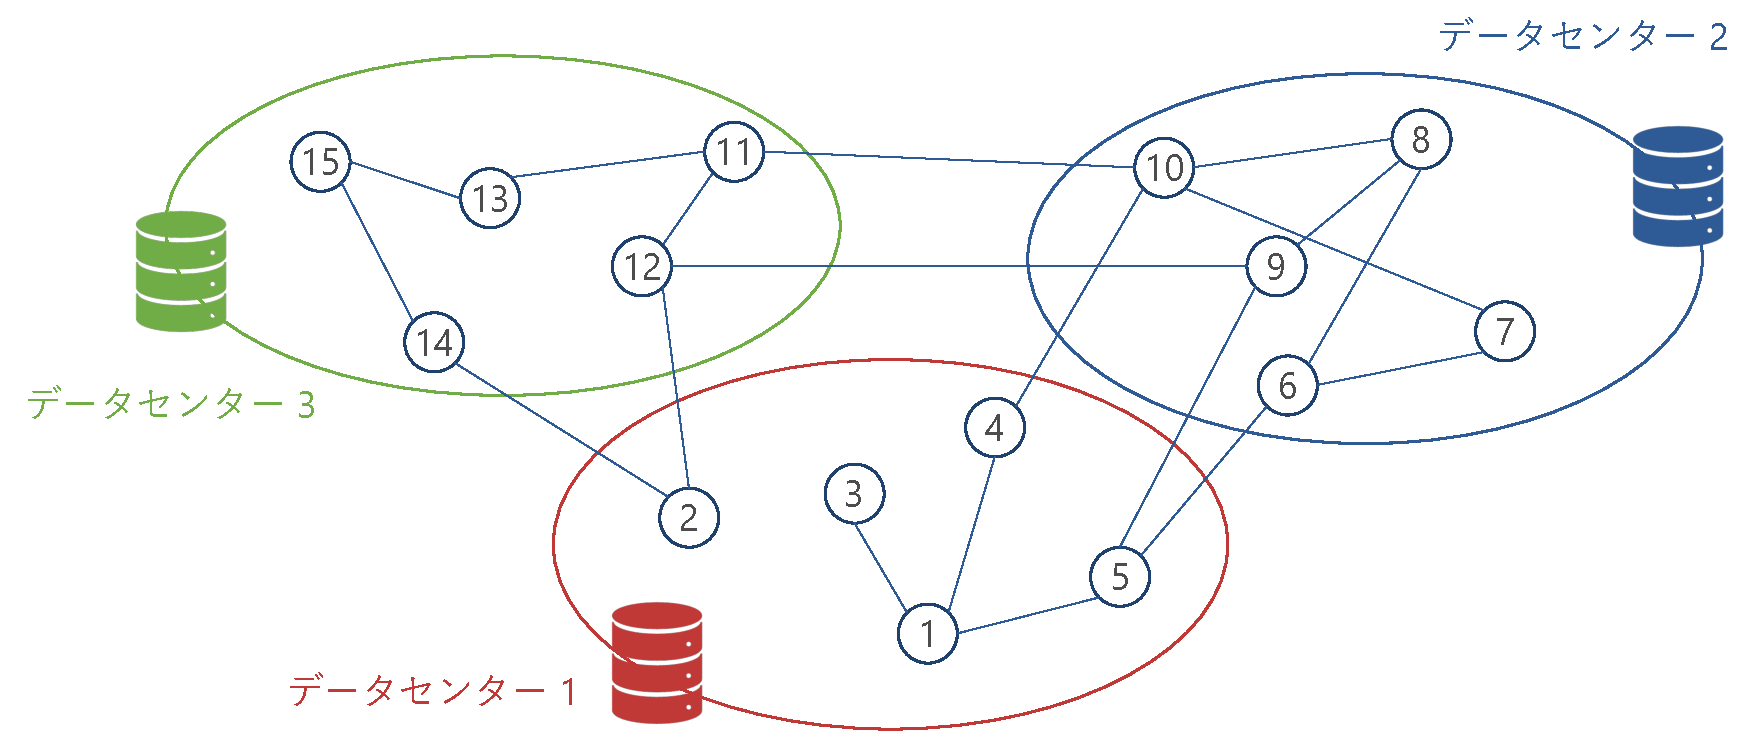
\includegraphics[scale=0.5]{figure/dcgraph.pdf}
    \caption{地理的分散環境下におけるグラフ.}
    \label{地理的分散環境下におけるグラフ}
\end{figure}

\section{本論文の構成}

以降の本論文の構成を示す. まず第 \ref{chap:related_work} 章で関連研究について述べる. 第 \ref{chap:design} 章では本研究における提案手法について述べ, 第 \ref{chap:implement} 章では提案手法の実装について述べる. 第 \ref{chap:eval} 章では提案手法の評価について述べ, 最後に第 \ref{chap:conclusion} 章で本論文をまとめ, 今後の課題について述べる. 

\chapter{関連研究}
\label{chap:related_work}
本章では関連研究について, 本研究の構成要素である 「Random Walk エンジン」「分散グラフ処理システム」「地理的分散環境におけるグラフ処理システム」の 3 つに分けて紹介する. その後, 本研究の位置づけを述べる. 

\section{Random Walk エンジン}\label{sec:Random Walk エンジン}

Random Walk (RW) はグラフ解析において頻繁に用いられるため, その RW 演算を効率的に実行するシステムの開発は有意義なものであり, 複数の既存技術が存在する. 

ThunderRW\cite{10.14778/3476249.3476257}, FlashMob\cite{10.1145/3477132.3483575} は共有メモリシステムにおける RW 演算の最適化を目的とした手法である. RW 演算ではランダムな隣接頂点への遷移を繰り返すため, 不規則なメモリアクセスが課題となる. そこで ThunderRW では異なる RW クエリの実行を切り替えることによりメモリアクセスの待ち時間を隠蔽した. また FlashMob では, Random Walker (RWer) は高次数頂点に高頻度で訪れることに注目し, 高次数頂点の隣接辺の事前サンプリングを行うことで, RWer の遷移を DRAM への Sequential Read に置き換え, メモリアクセスのオーバヘッドを削減した. 

DrunkardMob\cite{10.1145/2507157.2507173}, GraphWalker\cite{254449}, NosWalker\cite{10.1145/3582016.3582025} はシングルマシンで動作する Out-of-Core RW エンジンである. Out-of-Core RW エンジンでは, 全てのグラフデータをメモリに載せて演算を行うのではなく, 必要なグラフデータを逐一メモリにロードしながら RW 演算を実行する. DRAM に対して低価格である SSD を利用してグラフデータを保持するため, 大規模グラフ上における RW 演算をより低コストで実行することが可能になる. NosWalker では, エッジサンプリングはエッジデータのみ, walker のアップデート処理は頂点データのみが必要となる RW の特性に注目し, それぞれの処理を分離する walker 指向の非連結アーキテクチャを採用している. 
% 最先端手法である NosWalker は, 汎用的な Out-of-Core グラフ処理フレームワークをベースとしている DrunkardMob, GraphWalker に対し, RW の特性を活かしたアーキテクチャを採用している.

KnightKing\cite{10.1145/3341301.3359634} はグラフデータを分散クラスタ上で保持する分散グラフ RW エンジンである. KnightKing には汎用性の高い API が設定されており, PPR, DeepWalk, MetaPath, Node2vec といった複数種類の RW を実行することができる. さらに KnightKing の貢献として, rejection ベースのエッジサンプリング手法による, 高次 RW アルゴリズムのコスト削減がある. RW 演算のボトルネックはエッジのサンプリング処理にあると言われており, walker の現在の状態, 前回訪れた頂点, 現在滞在している頂点のエッジの性質に依存するような動的サンプリングを必要とする高次 RW は顕著にその傾向を示している. KnightKing の rejection ベースのエッジサンプリングは O(d) (d: 頂点における次数)かかっていたエッジの動的サンプリングを O(1) (前計算 O(n), n: 頂点数) に削減した.

\section{分散グラフ処理システム}\label{sec:分散グラフ処理システム}

近年のグラフデータの増加に伴い, 分散クラスタ上で動作する分散グラフ処理システムの重要性が高まっている. 分散グラフ処理における主流なプログラミングモデルとして, Bulk Synchronous Parallel (BSP) モデルがある. BSP モデルは, スーパーステップと呼ばれる単位で処理を繰り返し行うモデルであり, このスーパーステップは主に
\begin{itemize}
    \item サーバごとでの計算
    \item サーバ間同期
\end{itemize}
で構成される. 同期型である BSP モデルを非同期型にすることで処理を高速化する手法も存在する\cite{BAP}\cite{AAP}\cite{Gluon-Async}が, 実装の複雑化や, データセンター内等の広帯域環境では同期のオーバヘッドがさほど大きくならないことから, BSP モデルが採用されることが多い. 

BSP モデルの分散グラフシステムのうち, 頂点の状態に注目した手法\cite{Pregel}\cite{10.1145/2741948.2741970}\cite{10.5555/2387880.2387883}\cite{10.5555/3026877.3026901}\cite{Gluon}は vertex-centric なモデルと呼ばれる. vertex-centric モデルにおける各スーパーステップでは, 各頂点が, 直前のスーパーステップで送られたメッセージに基づいて自身の状態を更新し, 結果を他の頂点に送信する. ユーザは頂点における更新に関する処理を記述するのみであり, PageRank, Single Source Shortest Path, connected components 等の多くのグラフアルゴリズムはこの vertex-centric の形で書き下すことが可能である. 

対して\ref{sec:Random Walk エンジン} 節で紹介した KnightKing は, 処理単位が RWer であることから walker-centric モデルと呼ばれている. 図\ref{walker centric モデル (同期型) の概要} は walker-centric モデルの概要を示しており, 各スーパーステップでは, 
\begin{itemize}
    \item 各 RWer がユーザー定義の RW を実行 (1 ステップ進める) し, 状態を更新
    \item 状態を更新した RWer の内, 他のサーバが管理する頂点へ遷移した RWer を送信し, 全サーバで同期
\end{itemize}
を行う. vertex-centric モデルを採用しないのは, RW における RWer の概念は, 既存の vertex-centric モデルのシステムではメッセージとして扱われるため, RWer の状態更新の追跡や最適化のための機能が失われる可能性が高いためである. 

\begin{figure}[t]
    \centering
    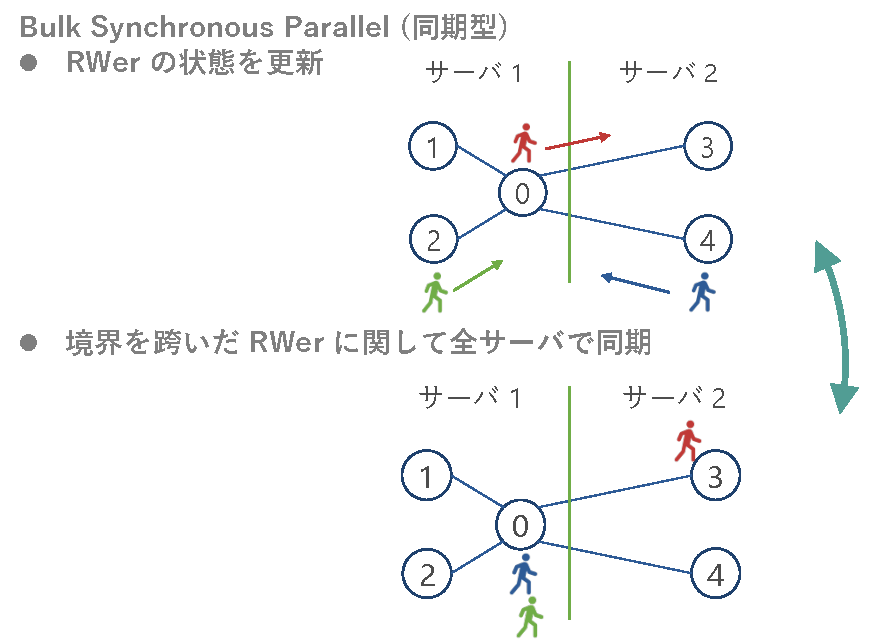
\includegraphics[scale=0.7]{figure/walkercentric.pdf}
    \caption{walker centric モデル (同期型) の概要}
    \label{walker centric モデル (同期型) の概要}
\end{figure}

\section{地理的分散環境におけるグラフ処理システム}

% 地理的に分散した環境でグラフデータが生成, 管理される状態を想定したグラフ解析システム\cite{10.5555/3277180.3277185}\cite{8486361}\cite{10.1145/3397271.3401157}も存在する. 
グラフクエリは, PageRank Web 検索\cite{334}, SNS 検索\cite{10.5555/2535461.2535468}, ナレッジグラフ検索\cite{10.1145/3331184.3331252}など, 多くの一般的なインターネットサービスの基盤となっているが, このようなグラフクエリで処理されるグラフは巨大であり, 変化の速度も速い\cite{10.1145/2723372.2735365}ため, 広域ネットワーク (WAN) でのデータ転送のコストが高い. さらに GDPR 等のプライバシー規制も相まって, グラフデータ全体を一箇所に集めることは極めて困難である. そのため, 地理的に分散した環境下における効率的なグラフ処理システムの開発が重要となる. 

\ref{sec:分散グラフ処理システム} 節で紹介した分散グラフ処理システムは, 単一のデータセンター内のサーバクラスタのような高帯域・低遅延な環境下で実行することを想定しているため, 低帯域・高遅延の WAN での実行では大きく性能が劣化する. これは BSP モデルのスーパーステップにおける隣接ノード間の通信がアルゴリズムの収束まで何度も繰り返されるからである. 

そこで, 既存の地理的分散環境下を想定した分散グラフ処理システム\cite{10.5555/3277180.3277185}\cite{8486361}\cite{10.1145/3397271.3401157} は \ref{sec:分散グラフ処理システム} における一般的な vertex-centric モデルの通信削減に注力している. HSP モデル\cite{8486361} では, サーバ間の同期をデータセンター内とデータセンター間で 2 階層に分けることにより, データセンター間での通信量を削減する. また, GeoGraph\cite{10.1145/3397271.3401157} では, WAN レイテンシに基づきデータセンターをグループ化し, そのグループ間の通信量を削減する. どちらも低帯域・高遅延な部分の通信削減を目的としていることがわかる. 

\section{本研究の位置づけ}

まず, Random Walk エンジンとしての本研究の位置づけについて述べる. 図 \ref{Random Walk エンジンの分類} にマシン数と目的による Random Walk エンジンの分類を示す. 提案手法は, マルチマシンによる地理的分散環境下での実行を目的とした手法に分類される. ThunderRW, FlashMob 等のシングルマシンにおけるメモリアクセスの改善を目的とした手法は, グラフの変化に対応することができないため, 本研究が想定する地理的分散環境下への適用が困難である. DrunkardMob, GraphWalker, NosWalker は大規模グラフでの RW 実行をシングルマシンで行うことによりコストを抑えようとしているため, 分散環境を許容している本研究とは目的と手段がそれぞれ異なる. KnightKing は単一データセンターでの RW 実行を目的とした, 分散グラフ RW エンジンであり, TCP 通信による同期処理を採用している. しかし本研究が想定する地理的分散環境下では RTT・パケットロス率が高くなり, TCP 通信のスループットが大幅に低下するため, 同期のオーバヘッドが大きくなる. また, RW の特徴である終盤の少数の RWer のためにわざわざ同期処理を行うのは無駄が多い. 

次に分散グラフ処理システムとしての本研究の位置づけについて述べる. 図 \ref{分散グラフ処理システムの分類} に分散グラフ処理システムの分類を示す. 提案手法は, 地理的分散環境下における walker-centric モデルの手法に分類される. HSP モデル, GeoGraph は vertex-centric モデルにおける通信削減を目的としている. vertex-centric モデルの計算では, 頂点間の同期の順番を入れ替えることで, 値の収束を早めたりサーバ間の通信量を減らすことができるが, walker-centric モデルでは RWer の遷移先を変更できないためサーバ間の通信量を減らすことができない. つまり HSP モデル, GeoGraph を walker-centric モデルに 適用させることはできない. 

\begin{figure}[t]
    \centering
    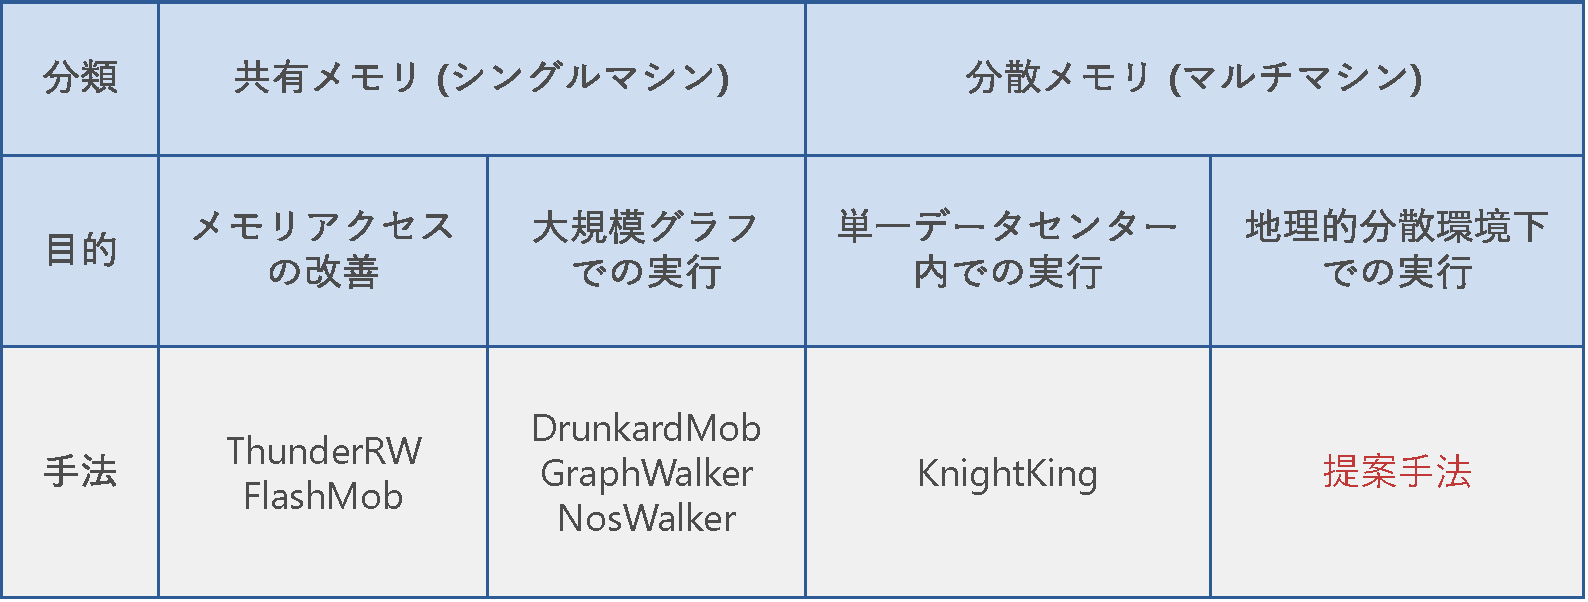
\includegraphics[scale=0.5]{figure/RWEngine.pdf}
    \caption{Random Walk エンジンの分類}
    \label{Random Walk エンジンの分類}
\end{figure}

\begin{figure}[t]
    \centering
    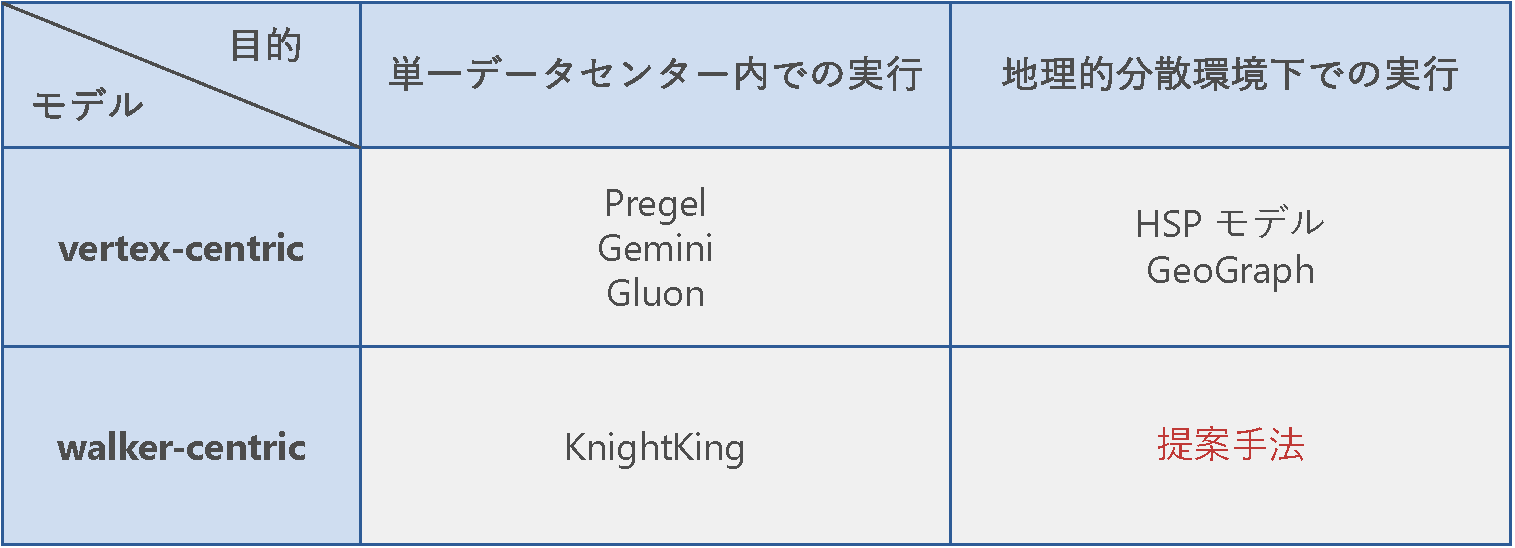
\includegraphics[scale=0.5]{figure/DistributedSystem.pdf}
    \caption{分散グラフ処理システムの分類}
    \label{分散グラフ処理システムの分類}
\end{figure}

\chapter{提案手法}
\label{chap:design}
本章では提案手法の詳細について述べる. まず \ref{概要} 節にて提案手法のアプローチについて述べる. 次に \ref{提案手法の全体像について} 節で提案手法の全体像について述べる. そして \ref{Random Walker の構成} 節にて, その後の説明で必要となる Random Walker の構成要素について述べ, \ref{Random Walker の経路再利用} 節で Random Walker の経路再利用について述べる.

\section{アプローチ}\label{概要}

提案手法は地理的に分散した環境における Random Walk (RW) エンジンであるため, 地理的分散環境下での RW 演算の特徴に合わせた実行形態を採用する. 

まず, 提案手法は同期処理を採用していた既存手法とは異なり非同期処理を採用する. 図 \ref{walker centric モデル (非同期型) の概要} に提案手法における非同期処理の概要を示す. 図 \ref{walker centric モデル (同期型) の概要} が示す同期型の手法とは異なり, RWer が他のサーバが所有する頂点に遷移した時点で他のサーバを待たずに送信を行う. 理由は 2 つある. 
% 1 つ目は地理的分散環境下における RW エンジンの用途である. 今後グラフがより大規模化していくことを考慮すると, 全世界に分散するグラフ上の全頂点から RW を実行することは現実的ではなく, 興味がある 1 部頂点を始点とした RW の実行が主流になると考える. この RW 実行はおそらくデータセンターごとに独立して行われる. つまり, 各データセンターが, 自身が保有する頂点を始点とした RWer の生成・ 処理を自律的に行い, その RW 結果をそのデータセンターの所在地域が活用することとなる. このような用途を考え, 地理的分散環境下における RW エンジンは各地域のデータセンターごとでの非同期処理が妥当であると判断した. ただし本研究では, 簡単のため 1 つのデータセンターを 1 つのサーバと見立てている. 
1 つ目は地理的分散環境下における RW エンジンの用途である. 今後グラフがより大規模化していくことを考慮すると, 全世界に分散するグラフ上の全頂点から RW を実行することは現実的ではなく, 興味がある 1 部頂点を始点とした RW の実行が主流になると考える. この RW 実行はおそらくデータセンターごとに独立して行われる. つまり, 各データセンターが, 自身が保有する頂点を始点とした RWer の生成・ 処理を自律的に行い, その RW 結果をそのデータセンターの所在地域が活用することとなる. この自律的な RW 実行を同期処理で実現する場合, 世界中の全データセンターが一つのデータセンターの一つのアプリケーション内の RW のために同期を行う必要がある. 地理的分散環境下のような低帯域・高遅延の環境 (WAN) ではこの同期のために何度も発生する通信のオーバヘッドがさらに増加する. また, 地理的分散環境下におけるグラフ編集によるグラフ分割の精度低下によって, サーバ間を跨ぐ RWer が増加するため, 同期の回数が増えてしまう. さらに, データセンターが増加するとその分同期の負担が大きくなるため, スケーラビリティが低い. そのため, 地理的分散環境下における RW エンジンは各地域のデータセンターごとでの非同期処理が妥当であると判断した. ただし本研究では, 簡単のため 1 つのデータセンターを 1 つのサーバと見立てている. 

2 つ目は RW 処理は RWer 単位で独立していることである. RW は PageRank, Single Source Shortest Path 等の一般的なグラフアルゴリズムとは異なり繰り返し実行されるため, 各試行は独立している. そのため, RWer 間での同期は必要ない. 逆に PageRank 等の一般的なグラフアルゴリズムは, 実行途中における各頂点に割り振られた値が互いに作用し合うため, 逐一同期を行う必要があることが多い. 
% 3 つ目は WAN での同期コストが大きいことである. 同期処理をする場合, 全サーバで同期のための通信が何度も発生するが, WAN のような低帯域・高遅延の環境下ではその通信のオーバヘッドが大幅に増加する. 

\begin{figure}[t]
    \centering
    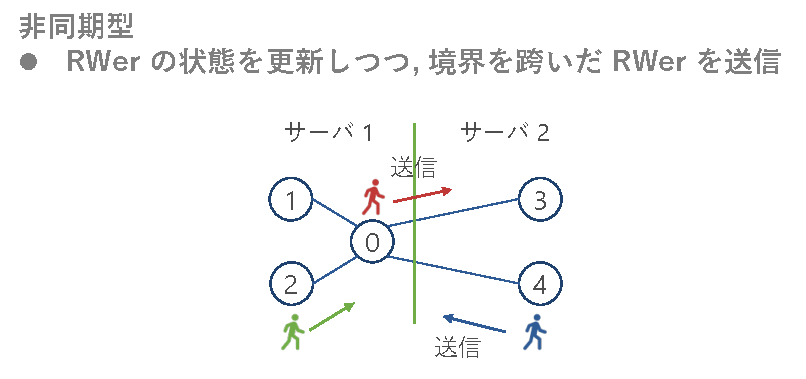
\includegraphics[scale=0.8]{figure/walkercentric_async.pdf}
    \caption{walker centric モデル (非同期型) の概要.}
    \label{walker centric モデル (非同期型) の概要}
\end{figure}

\begin{figure}[t!]
    \centering
    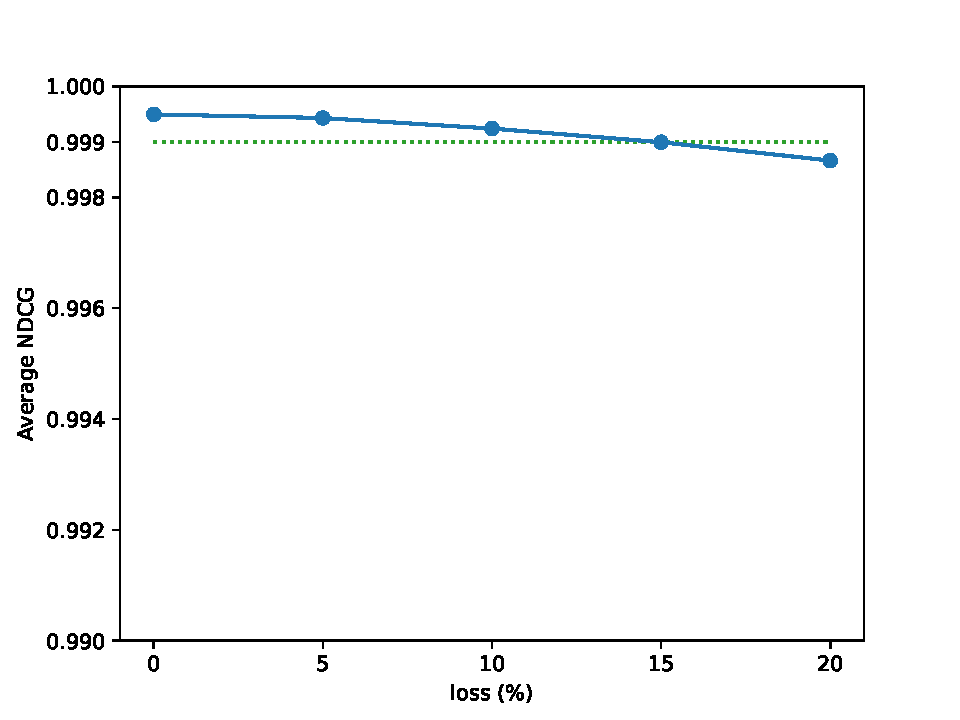
\includegraphics[scale=0.7]{figure/eva_drop.pdf}
    \caption{局所的に RWer が損失したときの PPR 演算の精度.}
    \label{局所的に RWer が損失したときの PPR 演算の精度}
\end{figure}

次に, 提案手法は RWer の送受信に UDP 通信を採用する. UDP 通信では, たとえ RTT・パケットロス率が高かったとしてもデータ転送スピードに影響しない. そのため, 地理的分散環境下における RWer の送受信には UDP 通信が適している. UDP 通信のデメリットはパケットロスが発生することであるが, RW の独立性により, RWer の損失のデメリットは少ない. 図 \ref{局所的に RWer が損失したときの PPR 演算の精度} に局所的に RWer が損失したときの Personalized PageRank (PPR) 演算の精度を示す. PPR とは, ある始点から始めた RW における各頂点の滞在確率を表している. この実験では LiveJournal のデータセット\cite{snapnets} のグラフを 5 台のサーバで分散管理し, ランダムな開始頂点から 50000 回の RW を実行することで RWer の経路情報から PPR を計算した. ここで, サーバ 1, 2, 3, 4 からサーバ 5 への RWer の送信の $x\%$ (図 \ref{局所的に RWer が損失したときの PPR 演算の精度} の横軸) を意図的に落とすことで, RWer が局所的に損失するシミュレーションを行った. PPR 演算精度を NDCG と呼ばれる指標で算出し, ランダムな開始頂点 1000 個分の平均を 図 \ref{局所的に RWer が損失したときの PPR 演算の精度} の縦軸に設定した. NDCG は 1 に近づくほど精度が高くなり, 0.999 程度あれば真値とほとんど等しい. NDCG が 0.999 を下回るのは意図的に落とす確率が 15 $\%$ のときであるため, RWer の損失が RW を利用したアプリケーションへ及ぼす影響は少ないことがわかる. 

UDP 通信の他にも QUIC と呼ばれる UDP 通信を用いて高速化しつつ TCP 通信のような通信の信頼性を提供するトランスポート層のプロトコルがある. UDP 通信に対する QUIC のメリットは, 認証・暗号化による安全性, そして再送制御による信頼性である. しかし本研究において, 安全性は現時点では不必要であり, 図 \ref{局所的に RWer が損失したときの PPR 演算の精度} のようにパケットロスの影響が少ないため再送制御も不必要である. そのため本研究では QUIC ではなく UDP 通信を採用した. 

また, 提案手法は終了した RWer の経路再利用により, RW 遷移における RWer 送受信を一部スキップする. 地理的分散環境下における RW 実行でボトルネックとなるのはサーバを跨ぐ RW 遷移による RWer の送受信である. そのため, この機能を導入することで実行時間を削減することができる. 

\section{提案手法の全体像}\label{提案手法の全体像について}

本節では提案手法の全体像について述べる. 図 \ref{提案手法の全体像} に提案手法の全体像を示す. 各サーバは独立して RWer 生成, RW 処理, 送信, 受信を自律的に行う. RW 処理では, 生成した RWer, 受信した RWer を滞在頂点からランダムに遷移させ続ける. このとき他のサーバが保持する頂点への遷移が発生した場合は, その RWer を頂点の持ち主サーバへ送信する. また, 途中で RW が終了した場合は RWer をその RWer の生成サーバへ送信する. このシステムを使用するユーザーはまず, 興味のある頂点を始点とする RWer の生成をシステムに命令し, RW 実行を開始する. その後終了して帰ってきた RWer をグラフの解析に利用することとなる. RWer の経路再利用機能では, この帰ってきた RWer の経路情報を保存しておき, 次回以降の RW 遷移に活用する. 

\begin{figure}[t]
    \centering
    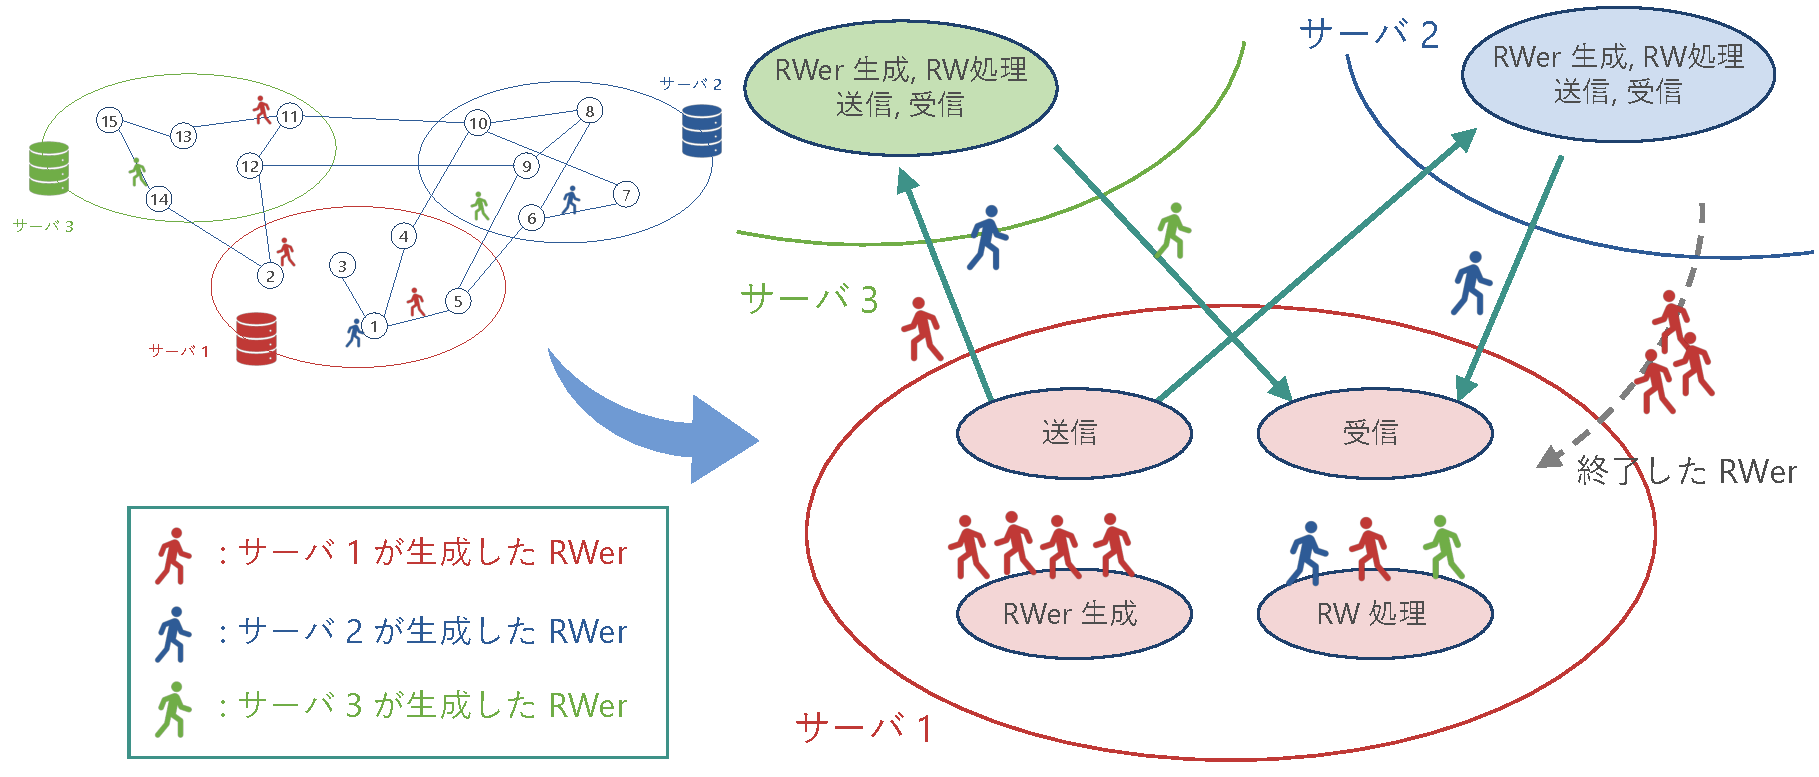
\includegraphics[scale=0.5]{figure/proposed.pdf}
    \caption{提案手法の全体像.}
    \label{提案手法の全体像}
\end{figure}

\section{Random Walker の構成}\label{Random Walker の構成}

本節では提案手法における RWer の構成について述べる. 表 \ref{RWer の構成} に RWer の構成を示す. $ver\_id\_$ はバージョンとメッセージ ID を含んでおり, メッセージ ID によって, 生存している RWer or 終了した RWer or 複数の RWer が入っているメッセージを識別する. この $ver\_id\_$ はメッセージの送受信におけるパケットにも付与するがその詳細については \ref{chap:implement} 章で述べる. $flag\_$ では RW 処理をする上で必要となる情報をフラグとして保持する. 1 hop 前で通信が発生したかを保持しておくことで, その遷移先で経路情報における通信発生フラグを立てることができる. また, $next\_index\_$ に値が入っているかを保持しておくことで, \ref{Random Walker の経路再利用} 節で説明する送信先での index による遷移を行うことができる. そして全体を通して通信が発生したかを保持しておくことで, 終了した RWer を他のサーバに送信するかどうかを判断することができる. $RWer\_size\_$ は RWer 単体のメモリサイズを保持する. これはメッセージ送信時の複数の RWer をまとめる際に必要となる. $RWer\_id\_$ は RWer の識別 ID である. $RWer\_life\_$ は RW 演算における残り hop 数を保持する. 提案手法では RWer 生成時に経路長を先に計算する. 例えば各遷移ごとで確率 $\alpha (< 1)$ で終了する RW 演算であれば, $0 < r < 1$ の乱数を $r < \alpha$ となるまで生成し, その生成回数を経路長とする. この $RWer\_life\_$ はサーバ上で RWer の構造体を生成する際, 可変長配列である $path\_$ のメモリ確保に使用される. $path\_length\_at\_current\_host\_$ は RWer の現在の同一ホスト内における経路長を保持する. これは $path\_$ における現在ホスト情報の位置を特定する際に使用される. $next\_index\_$ は通信が発生したときの次の遷移先 index を示す. これは RWer の経路再利用機能で使用される. 

\begin{table}[t]
    \caption{RWer の構成.}
    \label{RWer の構成}
    \centering
    \begin{tabular}{ccc}
        \hline \hline
        名称  &  サイズ  &  内容 \\
        \hline 
        $ver\_id\_$  &  8 bit  &  バージョン: 4 bit, メッセージ ID: 4 bit \\
        \hline
        $flag\_$  &  8 bit  & 
        \begin{tabular}{c} 1 hop 前で通信が発生したか: 1 bit, \\$next\_index\_$ に値が入っているか: 1 bit, \\全体を通して通信が発生したか: 1 bit, \\予備: 5 bit 
        \end{tabular}\\
        \hline
        $RWer\_size\_$  &  16 bit  &  RWer 単体のメモリサイズ \\
        \hline
        $RWer\_id\_$  &  32 bit  &  RWer の識別 ID \\
        \hline
        $RWer\_life\_$  &  16 bit  &  RWer の残り歩数  \\
        \hline
        $path\_length\_at\_current\_host\_$  &  16 bit  &  RWer の現在の同一ホスト内の経路長  \\
        \hline
        $reserved\_$  &  32 bit  &  予備  \\
        \hline
        $next\_index\_$  &  64 bit  &  通信が発生したときの次の遷移先 index \\
        \hline
        $path\_$  &  64 bit の可変長配列  &  経路情報  \\
        \hline
    \end{tabular}
\end{table}

\begin{figure}[t]
    \centering
    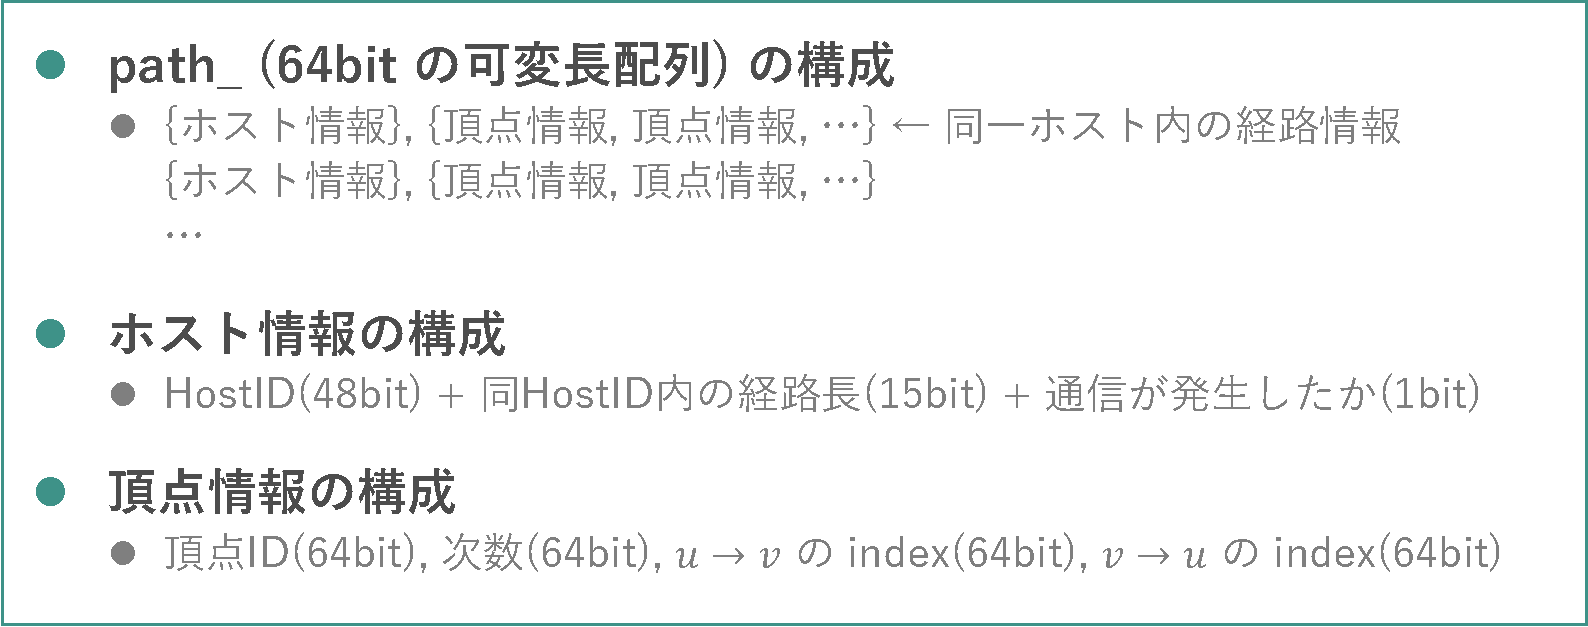
\includegraphics[scale=0.5]{figure/path.pdf}
    \caption{経路情報の構成.}
    \label{経路情報の構成}
\end{figure}

図 \ref{経路情報の構成} に $path\_$ (経路情報) の構成を示す. $path\_$ は, ホスト情報 (64 bit), 頂点情報 (64 bit $\times$ 4), 頂点情報, ... , ホスト情報, 頂点情報, ... のように頂点情報をホストごとにグループ化する. これにより各頂点情報にその頂点を保有するホストの情報を入れる必要がなくなり, サイズを削減することができる. ホスト情報の構成は, HostID (48 bit), 同一 HostID 内の経路長 (15 bit), 通信が発生したかどうかのフラグ (1 bit) である. 同一 HostID 内の経路長は経路情報を前方から探索していく際に必要となる. 通信が発生したかどうかのフラグは, 経路再利用による通信スキップが発生しなかった場合の判定に利用できる. 頂点情報の構成は, 頂点 ID (64 bit), 次数 (64 bit), $u \rightarrow v$ の index (64 bit), $v \rightarrow u$ の index (64 bit) である. $u \rightarrow v$ の index はひとつ前の頂点から見た今の頂点の index 情報であり, $v \rightarrow u$ の index は今の頂点から見たひとつ前の頂点の index 情報である. 逆方向の index 情報を保持しておくことで, 無向グラフにおける逆向きの経路情報も再利用することができる. 次数情報は経路再利用時に使用されるため頂点情報に含まれている.

\section{Random Walker の経路再利用}\label{Random Walker の経路再利用}

地理的分散環境下での RW 実行においてボトルネックとなるのは, サーバを跨ぐ RW 遷移における RWer の送受信である. 提案手法ではこの RWer の送受信を減らすため, RWer の経路再利用による通信スキップ機能を追加する. 図 \ref{RWer の経路再利用機能の概要} に RWer の経路再利用機能の概要を示す. 図の左上では, サーバ 1 上の頂点 1 を始点とする RW がサーバ 3 上の頂点 13 で終了した状態を表しており, その後サーバ 3 は終了した RWer を生成サーバであるサーバ 1 へ送信する. 生成サーバであるサーバ 1 は自身が所有するグラフとその周辺の解析のためにこの終了した RWer を利用するため, サーバ 3 からサーバ 1 への RWer 送信は RWer の経路再利用のためだけに追加した処理ではない. 図の右下は, サーバ 1 がサーバ 3 から RWer を受信した後での, サーバ 1 上の頂点 4 からサーバ 2 上の頂点 10 への RW 遷移を表している. 通常, 所有サーバが異なる頂点間の遷移では RWer の送受信が発生するが, 以前に受信した RWer の経路情報の一部 (頂点 10 の次数や index 情報) を利用することによって, サーバ 1 からサーバ 2 への送信をスキップすることができる. 本手法における RW 遷移の一般的な手順は Algorithm \ref{RW 遷移} に示す.

\begin{figure}[t]
    \centering
    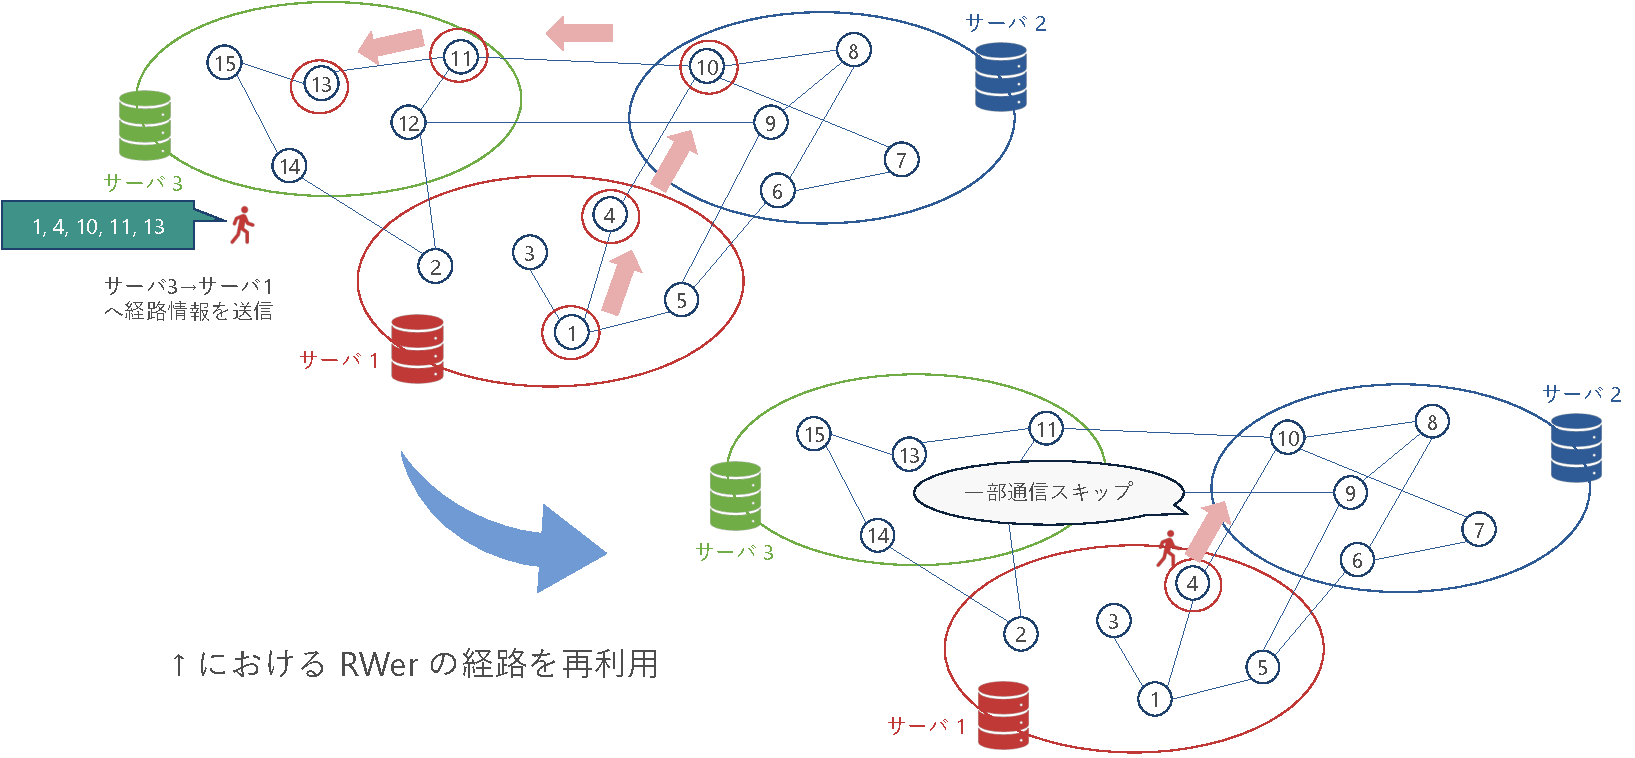
\includegraphics[scale=0.5]{figure/cache_gai.pdf}
    \caption{RWer の経路再利用機能の概要.}
    \label{RWer の経路再利用機能の概要}
\end{figure}

\begin{algorithm}[t]
\DontPrintSemicolon
\nl     $v \leftarrow$ RWer が滞在している頂点\;
\nl     \If{$v$ が自サーバの所有頂点である} {
\nl         \If{RWer に次の遷移先の index 情報が格納されている} {
\nl             その情報通りに RWer を遷移させる\;}
\nl         \Else {
\nl             ランダムに遷移\;}}
\nl     \ElseIf{$v$ が自サーバの所有頂点でない} {
\nl         $degree \leftarrow$ 過去の経路情報から得られた $v$ の次数\;
\nl         $next\_index \leftarrow 0 \leq r < degree$ のランダムな値\;
\nl         $next\_node \leftarrow v$ の $next\_index$ 番目の隣接頂点\;
\nl         \If{$next\_node$ が過去の経路情報から得られなかった場合} {
\nl             $RWer$ に $next\_index$ の情報を格納し, $v$ の持ち主サーバへ送信\;}
\nl         \Else {
\nl             $RWer$ を $next\_node$ に遷移させる (通信スキップ)\;}}
\caption{{RW 遷移} \label{RW 遷移}}
\end{algorithm}

図 \ref{具体例における RWer の経路情報} は図 \ref{RWer の経路再利用機能の概要} の RWer の経路情報を具体的に示したものである. 頂点の周りに記載されている数字は index 情報を示している. 例えば頂点 1 から見た頂点 4 の index は 1 となる. この index 情報は頂点 ID の昇順で各頂点に振り分けられる. サーバ 3 での RW 終了時, RWer はサーバ 1 へ送信されるため, サーバ 1 がこの経路情報を保有する. 図 \ref{経路再利用による送信スキップ} に経路再利用による送信スキップの詳細を示す. サーバ 1 上で頂点 4 から頂点 10 への遷移が決まった後, サーバ 1 は経路情報から頂点 10 の次数が 4 であることを知っているため, 頂点 10 の次の遷移先 index をランダムに選択する. 遷移先 index が 0, 3 の場合は経路情報からそれぞれ頂点 4, 頂点 11 へ遷移することがわかるため, サーバ 1 上で遷移を行う. 遷移先 index が 1, 2 の場合は経路情報から遷移先がわからないため, サーバ 2 へ送信することになる. このとき, 表 \ref{RWer の構成} の $next\_index\_$ に index 情報を格納する. そしてサーバ 2 が RWer 受信したのち, この index 情報を利用して RW の遷移を行う. この例では頂点 4 から頂点 10 への遷移におけるサーバ間の RWer 送信が 4 分の 2 の確率でスキップされることになる. サーバ 1 上で頂点 10 から頂点 11 への遷移が決まった場合は, 頂点 11 からの遷移に関しても頂点 10 と同様にしてその先の遷移を行うことができる. 

\begin{figure}[t]
    \centering
    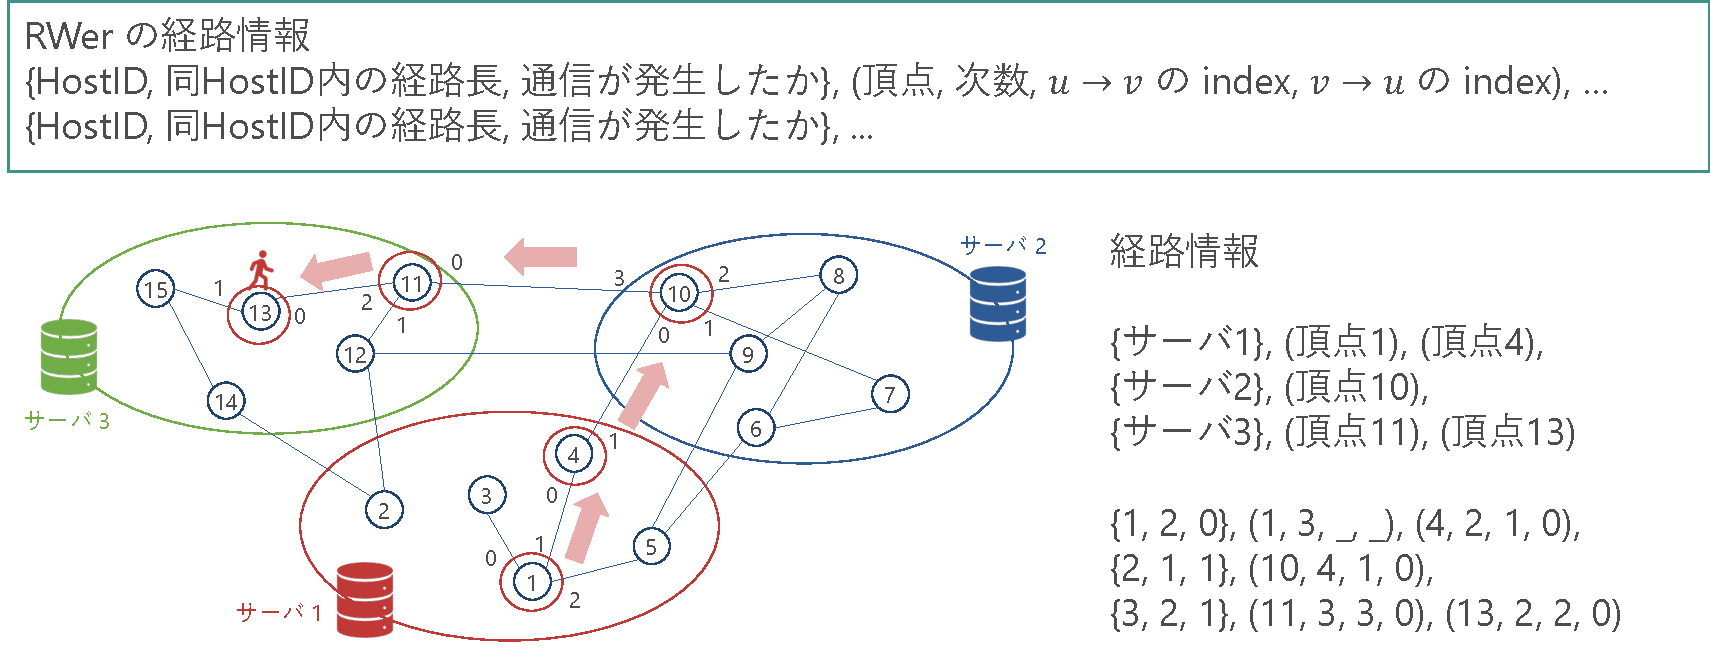
\includegraphics[scale=0.5]{figure/path_ex.pdf}
    \caption{具体例における RWer の経路情報.}
    \label{具体例における RWer の経路情報}
\end{figure}

\begin{figure}[t]
    \centering
    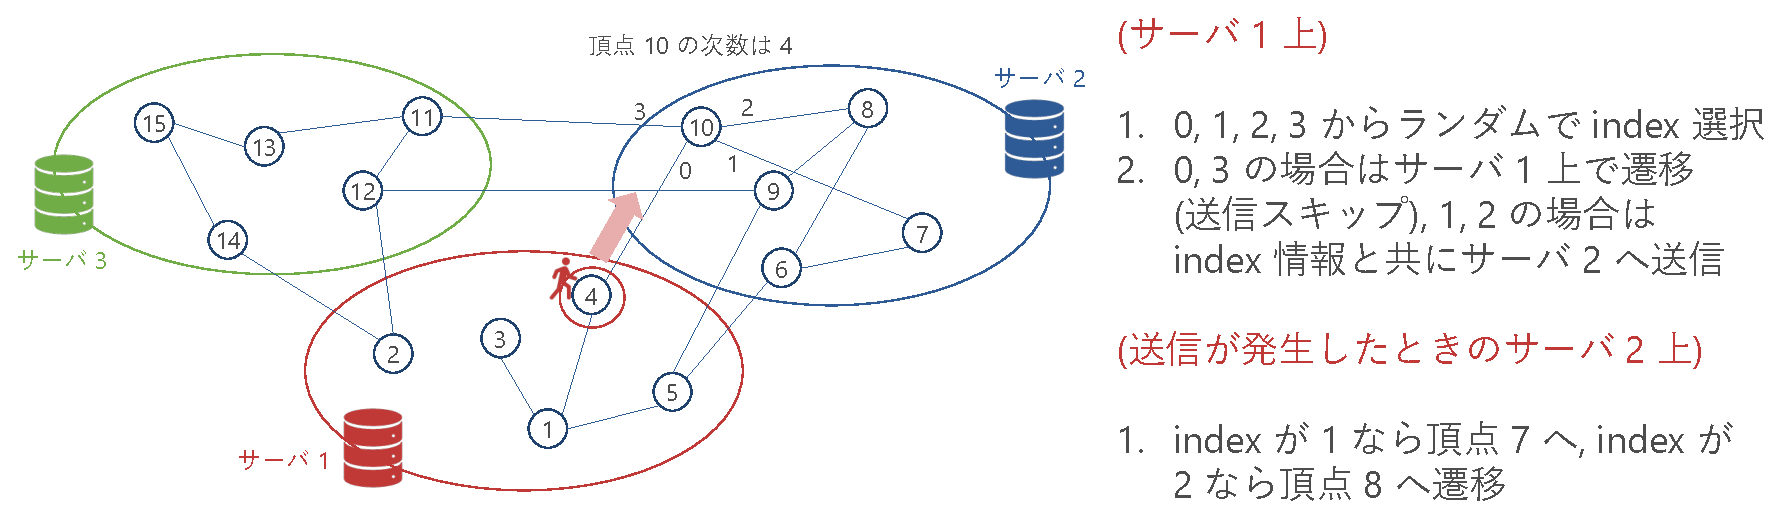
\includegraphics[scale=0.5]{figure/skip.pdf}
    \caption{経路再利用による送信スキップ.}
    \label{経路再利用による送信スキップ}
\end{figure}

% \section{実装}\label{実装}

% 本節では提案手法の実装について述べる. 図 \ref{サーバ上の実装の概要} に実装の概要を示す. 提案手法はサーバクラスタによる分散グラフ処理システムであるため, 各サーバ上でこの実装によるプログラムが動作する. RWer 生成 \& 処理スレッドでは, RWer を生成しその後 RW 処理を行う. このとき他のサーバが所有する頂点への遷移が発生した場合は, その RWer を送信キューに格納する. 受信スレッドでは, 他のサーバからメッセージを受信し, そのメッセージの種類に応じた処理を行う. 例えばメッセージが複数の RWer を含むものだった場合は, それらの RWer を RWer キューに格納する. RWer 処理スレッドでは, RWer キューから RWer をまとめて取り出し, RW 処理を行い, 他のサーバが所有する頂点への遷移が発生した場合は, その RWer を送信キューに格納する. 送信スレッドでは, 送信先ごとの送信キューから RWer をまとめて取り出し, 他のサーバへ送信する. 以降, 終了した Random Walker の経路情報の保持方法, 受信スレッド, RWer 処理スレッド, 送信スレッドの 4 つについて, 適宜擬似コードを用いて詳細を説明する. 

% \begin{figure}[t]
%     \centering
%     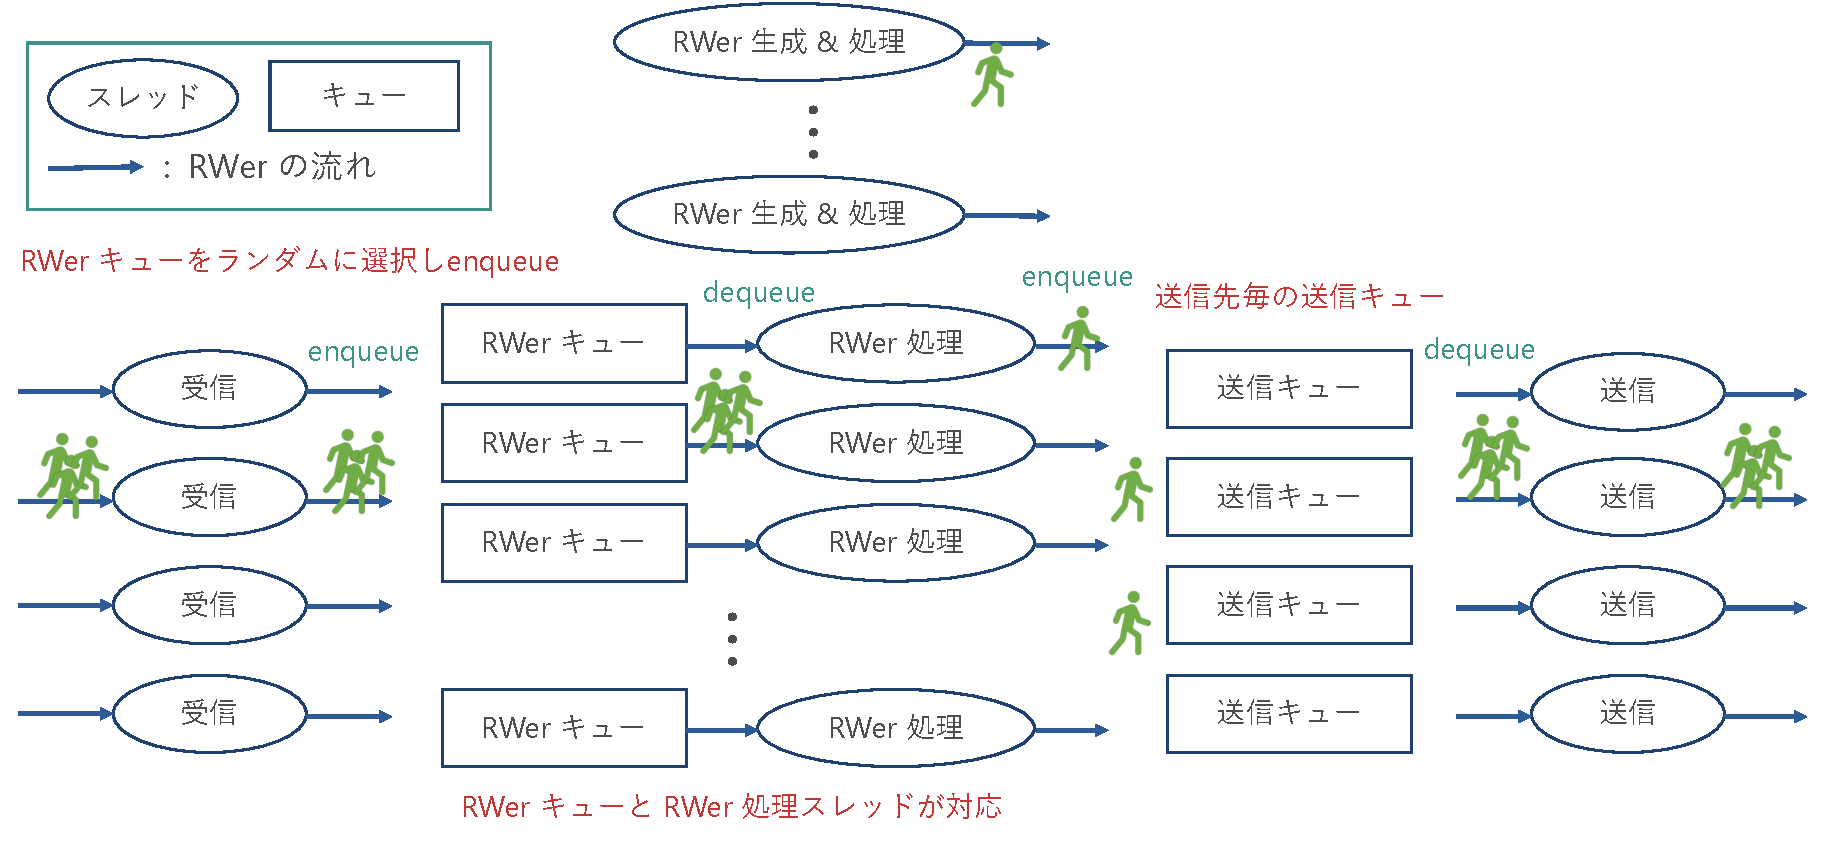
\includegraphics[scale=0.5]{figure/implementation.pdf}
%     \caption{サーバ上の実装の概要}
%     \label{サーバ上の実装の概要}
% \end{figure}

% \subsection{終了した Random Walker の経路情報の保持方法}

% \ref{Random Walker の経路再利用} で説明したように, 本手法では終了した RWer の経路情報を再利用することで通信のスキップを行う. そのためには終了した RWer の経路情報を保存しておく必要がある. 経路情報のまま保存するのは無駄が多いため, 経路再利用時に必要となる項目ごとに情報を保存する. 表 \ref{Random Walker の経路情報の保存形式} に RWer の経路情報の保存形式を示す. 本手法は C++ を使って実装しているためデータ構造は C++ の形式で記述した. 頂点に対する次数は RW 遷移時における index 選択の際に必要となる. データ構造に関しては, 頂点 ID を index とした配列の形で保持する. 頂点に対する持ち主サーバは, もし次の遷移先情報を持っていない場合に現在頂点の持ち主サーバへの RWer の送信が発生するため, 必要である. データ構造に関しては次数情報と同様, 頂点 ID を index とした配列の形で保持する. エッジデータは index を使った RW 遷移に必要となる. 例えば図 \ref{経路再利用による送信スキップ} ではサーバ 1 が (10, 0, 4), (10, 3, 11) (始点頂点, index, 遷移先頂点) というエッジデータを保持しているため, index = 0, 3 の場合は通信をスキップすることができる. データ構造に関しては, 頂点 ID を index とし, それぞれの頂点について (key, value) = (index, 遷移先頂点) のハッシュ map を保持する形とした. 

% \begin{table}[t]
%     \caption{Random Walker の経路情報の保存形式}
%     \label{Random Walker の経路情報の保存形式}
%     \centering
%     \begin{tabular}{cc}
%         \hline
%         保存項目  &  データ構造 (C++)  \\
%         \hline \hline
%         頂点に対する次数  &  std::vector$\langle$uint64$\_$t$\rangle$ \\
%         \hline
%         頂点に対する持ち主サーバ  &  std::vector$\langle$uint64$\_$t$\rangle$  \\
%         \hline
%         エッジデータ  &  std::vector$\langle$std::unordered$\_$map$\langle$uint64$\_$t, uint64$\_$t$\rangle$$\rangle$ \\
%         \hline
%     \end{tabular}
% \end{table}

% \subsection{受信スレッド}

% \begin{algorithm}[t]
% \DontPrintSemicolon
% \nl $message \leftarrow$ 受信データ\;
% \nl $message\_id \leftarrow message$ の先頭から抜き出した値\;
% \nl \If{$message\_id ==$ 複数の RWer によるメッセージ} {
% \nl     $RWer\_count \leftarrow message$ の先頭から抜き出した値\;
% \nl     $RWer \;\; A[RWer\_count]$\;
% \nl     $idx \leftarrow message$ 内における先頭の RWer 情報の開始位置\;
% \nl     \For{$i = 1$ to $RWer\_count$} {
% \nl         $A[i] \leftarrow message 内における i$ 個目の RWer の情報\;
% \nl         $idx \leftarrow idx$ + ($i$ 個目の RWer のメモリサイズ)\;}
% \nl     RWer キューをランダムに選択し, $A$ 内の RWer を全て格納\;}
% \nl \Else{
% \nl     他の場合は説明省略\;}
% \caption{{受信スレッド} \label{受信スレッド}}
% \end{algorithm}

% \begin{table}[t!]
%     \caption{メッセージの構成}
%     \label{メッセージの構成}
%     \centering
%     \begin{tabular}{ccc}
%         \hline
%         名称  &  サイズ  &  内容 \\
%         \hline \hline
%         $ver\_id\_$  &  8 bit  &  バージョン: 4 bit, メッセージ ID: 4 bit \\
%         \hline
%         $RWer\_count$  &  16 bit  &  メッセージ内に含まれる RWer の数 \\
%         \hline
%         複数の RWer  &  可変長サイズ $\times$ $RWer\_count$  &  表 \ref{RWer の構成} の RWer の情報を複数格納 \\
%         \hline
%     \end{tabular}
% \end{table}

% 受信スレッドでは, 他のサーバから受信したメッセージを処理し, 適宜 RWer を RWer キューに格納する. メッセージの種類は複数の RWer 以外にも実験開始の合図, 結果送信の合図等があるが, ここでは主要な処理である複数の RWer について説明する. Algorithm \ref{受信スレッド} に受信スレッドの擬似コードを示す. また, 提案手法におけるメッセージ構成を表 \ref{メッセージの構成} に示す. まず, 受信したメッセージを $message$ に格納し, $message\_id$ を先頭の $ver\_id\_$ から抽出する (1, 2 行目). 次に $message$ からメッセージ内の RWer の個数である $RWer\_count$ を抽出し, サイズ $RWer\_count$ の RWer 格納用配列を作成する (4, 5 行目). そしてその配列 $A$ に $message$ 内の RWer の情報を格納していく(6 -- 9 行目). $idx$ は $message$ 内におけるそれぞれの RWer の情報の開始位置を表す. つまり, 6 行目において $idx$ = 24 bit であり, RWer の情報の開始位置は先頭から 25 bit 目である. RWer の情報は可変長なので, 2 つ目以降の RWer に関する $idx$ については, その都度一つ前の RWer のメモリサイズを表 \ref{RWer の構成} の $RWer\_size$ から読み取り, 加算する(9 行目). 最後に, 格納先の RWer キューをランダムに一つ選択し, $A$ 内の RWer を全て格納する(10 行目). 本手法では, 並列性を可能な限り保つことができる構築を意識しており, 受信スレッドごとに異なるポート番号を振り分け, 受信処理を並列に行う. また, RWer 処理スレッドも同様で, 図 \ref{サーバ上の実装の概要} のように各 RWer スレッドごとに RWer キューを用意した. 10 行目における RWer キューのランダム選択は, 各 RWer 処理スレッドの負荷分散のためである. また, $A$ 内の RWer それぞれに対してランダムな RWer キューを選択するのではなく, $A$ 内の全ての RWer をまとめて一つの RWer キューに格納するのは, RWer キューにて必要となる排他制御のロックを低減させるためである. 

% 本手法ではスレッド間での情報のやり取りが多い. 例えば, 受信スレッドと RWer 処理スレッド間では RWer キューを通じて RWer を受け渡す. ここでもし RWer を構造体のまま RWer キューへ push, または RWer キューから pull しようとすると, その都度構造体のメモリコピーが発生してしまいオーバヘッドが大きくなる. そのため本手法では情報の受け渡しをポインタで行う. また, スレッド間でのポインタの受け渡しには所有権の概念が存在するため, C++ におけるスマートポインタを利用してこの処理を実装した. 



% \subsection{RWer 処理スレッド}

% RWer 処理スレッドでは, RWer キューから RWer をまとめて取り出し, それぞれの RWer に対して RW 処理を行い, 他のサーバが所有する頂点への遷移が発生した場合は, その RWer を送信キューに格納する. Algorithm \ref{RWer 処理スレッド} に RWer 処理スレッドの擬似コードを示す. まず RWer キューから RWer をまとめて取り出し, 配列 $A$ に格納する(1, 2 行目). そして $A$ 内の各 $RWer$ について RW 処理を行う(3 -- 38 行目). RW 処理については, まず $RWer$ の $ver\_id\_$ (表 \ref{RWer の構成} 参照) から $message\_id$ を抽出し, それがもし終了した RWer のものだった場合, 終了した RWer に対する処理を行う(4 -- 6 行目). 終了した RWer に対する処理では主にその RWer の生成サーバに対応する送信キューへの push を行う. $message\_id$ が, まだ生存している RWer のものであった場合は, その RWer が終了 or 他のサーバが所有する頂点へ遷移し, 送信キューに格納されるまで処理を繰り返し行う(7 -- 38 行目). ここでの処理は $RWer$ の現在頂点である $current\_node$ (9 行目)が自サーバの所有頂点である場合とそうでない場合で異なる. $current\_node$ が自サーバの所有頂点である場合は, 基本的には自分が所持するグラフ上でのランダム遷移を行う. しかし 1 hop 前で通信が発生した, かつ $RWer$ の $next\_index\_$ (表 \ref{RWer の構成} 参照) に index 情報が格納されている場合は, 次の遷移はその index 情報を利用して行う(11 -- 14 行目). これは図 \ref{経路再利用による送信スキップ} の送信が発生したときのサーバ 2 上での処理に対応している. 遷移先 index のランダム選択は送信前に済ませているため, 送信先で再びランダム選択を行うと不正確な RW 遷移となってしまう. $current\_node$ が自サーバの所有頂点でない場合は, 過去の RWer の経路情報を利用して RW 遷移を行う. 22 行目における, 過去の経路情報から $current\_node$ の次数がわからない場合は, $current\_node$ が, 自分が所有する頂点の隣接頂点のうち, 他サーバが所有するかつまだ経路情報に含まれていない頂点であることがわかる. 本手法が想定する分散グラフ管理下では, 隣接頂点が他サーバの所有する頂点である場合, 自サーバはその頂点の ID と持ち主サーバの情報のみを保持するとしているため, $current\_node$ が自サーバの所有頂点でない (他サーバの頂点 ID 情報を持っている) かつ $current\_node$ の次数情報を持っていないという状態が存在する場合がある. このときは, $RWer$ を $current\_node$ の持ち主サーバへの送信キューへ push する(22, 23 行目). ここでは次数がわからず, index のランダム選択は行わない($RWer$ の $next\_index\_$ に値を入れない)ため, この $RWer$ を受信したサーバは, 11 行目における if 文を通過し, 通常のランダム遷移を行う. $current\_node$ の次数 ($degree$) が過去の経路情報からわかる場合, $degree$ 未満のランダムな値を $next\_index$ として, $current\_node$ の $next\_index$ 番目の隣接頂点を次の遷移先頂点 ($next\_node$) とする(26, 31, 32 行目). ここで, $next\_node$ が過去の経路情報から得られなかった場合は, $RWer$ の $next\_index\_$ に $next\_index$ を入れ, $current\_node$ の持ち主サーバへの送信キューへ push する(33 -- 35 行目). これは図 \ref{経路再利用による送信スキップ} において, サーバ 1 上で 1 or 2 の index を選択した場合に対応する. この RWer を受信したサーバは, 11 行目の if 分で引っかかり, index 情報による決定的な遷移を行う. $next\_node$ が過去の経路情報から得られた場合は, $RWer$ をその $next\_node$ に遷移させる(38 行目). 
% \\
% \\
% \\
% \\

% \begin{algorithm}[p]
% \DontPrintSemicolon
% \nl vector$\langle$RWer$\rangle$ $\; A$\;
% \nl $A \leftarrow$ RWer キューから RWer をまとめて取り出し, 格納\;
% \nl \For{$each \; RWer \in A$} {
% \nl     $message\_id \leftarrow RWer$ の $ver\_id\_$ から抽出\;
% \nl     \If{$message\_id ==$ 終了した RWer} {
% \nl         終了した RWer に対する処理\;}
% \nl     \ElseIf{$message\_id ==$ 生存している RWer} {
% \nl         \While{true} {
% \nl             $current\_node \leftarrow RWer$ の現在頂点\;
% \nl             \If{$current\_node$ が自サーバの所有頂点である場合} {
% \nl                 \If{1 hop 前で通信が発生した $\&\&$ 次の遷移先の index 情報が格納されている} {
% \nl                     $next\_index \leftarrow RWer の next\_index\_$\;
% \nl                     $next\_node \leftarrow$ $current\_node$ の隣接リストの $next\_index$ 番目の頂点\;
% \nl                     $RWer$ を $next\_node$ に遷移させる\;}
% \nl                 \ElseIf{$RWer$ の $RWer\_life\_$ が 0 \textbar\textbar $\;current\_node$ の次数が 0} {
% \nl                     終了した RWer に対する処理\;
% \nl                     break\;}
% \nl                 \Else {
% \nl                     $next\_node \leftarrow$ $current\_node$ のランダムな隣接頂点\;
% \nl                     $RWer$ を $next\_node$ に遷移させる\;}}
% \nl             \ElseIf{$current\_node$ が自サーバの所有頂点でない場合} {
% \nl                 \If{過去の経路情報から $current\_node$ の次数情報がわからない場合} {
% \nl                     $current\_node$ の持ち主サーバへの送信キューに $RWer$ を push\;
% \nl                     break\;}
% \nl                 \Else {
% \nl                     $degree \leftarrow$ 過去の経路情報から得られた $current\_node$ の次数\;
% \nl                     \If{$RWer$ の $RWer\_life\_$ が 0 \textbar\textbar $\;degree == 0$} {
% \nl                         終了した RWer に対する処理\;
% \nl                         break\;}
% \nl                     \Else {
% \nl                         $next\_index \leftarrow 0 \leq r < degree$ のランダムな値 $r$\;
% \nl                         $next\_node \leftarrow current\_node$ の $next\_index$ 番目の隣接頂点\;
% \nl                         \If{$next\_node$ が過去の経路情報から得られなかった場合} {
% \nl                             $RWer$ の $next\_index\_ \leftarrow next\_index$\;
% \nl                             $current\_node$ の持ち主サーバへの送信キューに $RWer$ を push\;
% \nl                             break\;}
% \nl                         \Else {
% \nl                             $RWer$ を $next\_node$ に遷移させる\;}}}}}}}
% \caption{{RWer 処理スレッド} \label{RWer 処理スレッド}}
% \end{algorithm}

% \subsection{送信スレッド}\label{sub:送信スレッド}

% 送信スレッドでは, 送信先ごとの送信キューから RWer をまとめて取り出し, メッセージを生成し,他サーバへ送信する. Algorithm \ref{送信スレッド} に送信スレッドの擬似コードを示す. 1 -- 3 行目は各送信スレッドがどの送信キューを選択するかを決める処理を表している. 本手法では送信キューが送信先ごとに生成されるのに対し送信スレッド数は最初から決まっているため, それぞれの送信スレッドはどの送信キューに格納されている RWer を送信するのかを決める必要がある. 送信スレッド間で同時に同じ送信キューが選択されることを防ぐため, 1 -- 3 行目は送信スレッド間での排他制御となっている. $id\_num\_$ は全送信スレッド間での共有変数であり, 暫定送信先 ID を示す. この $id\_num\_$ が自サーバのものでないかつ, 他のサーバが $id\_num\_$ 番目の送信キューを占有していない状態を満たすまで $id\_num\_$ をインクリメントする(1 -- 2 行目). 条件を満たす $id\_num\_$ が得られたらスレッド内変数である $send\_id$ に格納する(3 行目). その後, $send\_id$ 番目の送信キューから RWer をまとめて取り出し, 配列 $A$ に格納する. 6 行目以降は配列 $A$ 内の $RWer$ をできるだけまとめながら送信する処理を表している. $message$ は送信するメッセージを入れる変数, $RWer\_count$ は一つのメッセージ内に含まれる RWer の数, $now\_message\_size$ は現在のメッセージサイズを示しており(6 -- 8 行目), メッセージサイズの初期値は $ver\_id\_$ と $RWer\_count$ のサイズの合計である 24 となる (表 \ref{メッセージの構成}). 9 -- 20 行目の for 文ではメッセージに $RWer$ のデータを書き込んでいくが, その際メッセージサイズが指定された最大サイズを超えてしまう場合はデータ書き込みの前にメッセージ送信を行う. 送信時のポート番号については受信ポート番号からランダムに一つ選択し, 設定する. メッセージ送信後は $message$, $RWer\_count$, $now\_message\_size$ を初期値に戻す. 全ての $RWer$ のメッセージへの書き込みが終わった後, メッセージ内に $RWer$ が残っていた場合はその $message$ を送信する(21, 22 行目). 送信におけるメッセージの最大サイズについては, MTU - IP ヘッダ (20 byte) - UDP ヘッダ (8 byte) とする. 送信データサイズが MTU を超えるとパケット分割が発生し, パケットロス時の RWer 損失数が増えてしまうためである. 実験においては MTU を 9000 に設定しているため, 送信スレッドにおけるメッセージの最大サイズは 8972 byte となる. 

% \begin{algorithm}[t!]
% \DontPrintSemicolon
% \nl \While{$id\_num\_ == hostid\_ \;$ \textbar\textbar 他のサーバが $id\_num\_$ 番目の送信キューを占有している} {
% \nl     $id\_num\_ \leftarrow (id\_num\_ + 1)\; \%$ 送信キューの数\;}
% \nl $send\_id \leftarrow id\_num\_$\;
% \nl vector$\langle$RWer$\rangle$ $\; A$\;
% \nl $A \leftarrow send\_id$ 番目の送信キューから RWer をまとめて取り出し, 格納\;
% \nl $message \leftarrow$ 空のメッセージ\;
% \nl $RWer\_count \leftarrow 0$\;
% \nl $now\_message\_size \leftarrow $ sizeof($ver\_id\_$) + sizeof($RWer\_count$)\;
% \nl \For{$each \; RWer \in A$} {
% \nl     $RWer\_size \leftarrow RWer$ のメモリサイズ\;
% \nl     \If{$now\_message\_size + RWer\_size \geq $ メッセージの最大サイズ} {
% \nl         $message$ に $ver\_id\_$ と $RWer\_count$ を格納\;
% \nl         $port\_num \leftarrow$ 指定されたポート番号の中からランダム選択\;
% \nl         $message$ を $send\_id$ の送信先へ送信 (ポート番号は $port\_num$)\;
% \nl         $message \leftarrow$ 空のメッセージ\;
% \nl         $RWer\_count \leftarrow 0$\;
% \nl         $now\_message\_size \leftarrow $ sizeof($ver\_id\_$) + sizeof($RWer\_count$)\;}
% \nl     $RWer$ を $message$ に書き込む\;
% \nl     $RWer\_count \leftarrow RWer\_count + 1$\;
% \nl     $now\_message\_size \leftarrow now\_message\_size + RWer\_size$\;}
% \nl \If{$RWer\_count > 0$} {
% \nl     残った $message$ を上記と同様にして送信\;}
% \caption{{送信スレッド} \label{送信スレッド}}
% \end{algorithm}

% \chapter{実装}
% \label{chap:implement}
% 本章では提案手法の実装について述べる. 図 \ref{サーバ上の実装の概要} に実装の概要を示す. 提案手法はサーバクラスタによる分散グラフ処理システムであるため, 各サーバ上でこの実装によるプログラムが動作する. RWer 生成 \& 処理スレッドでは, RWer を生成しその後 RW 処理を行う. このとき他のサーバが所有する頂点への遷移が発生した場合は, その RWer を送信キューに格納する. 受信スレッドでは, 他のサーバからメッセージを受信し, そのメッセージの種類に応じた処理を行う. 例えばメッセージが複数の RWer を含むものだった場合は, それらの RWer を RWer キューに格納する. RWer 処理スレッドでは, RWer キューから RWer をまとめて取り出し, RW 処理を行い, 他のサーバが所有する頂点への遷移が発生した場合は, その RWer を送信キューに格納する. 送信スレッドでは, 送信先ごとの送信キューから RWer をまとめて取り出し, 他のサーバへ送信する. 以降, 終了した Random Walker の経路情報の保持方法, 受信スレッド, RWer 処理スレッド, 送信スレッドの 4 つについて, 適宜擬似コードを用いて詳細を説明する. 

\begin{figure}[t]
    \centering
    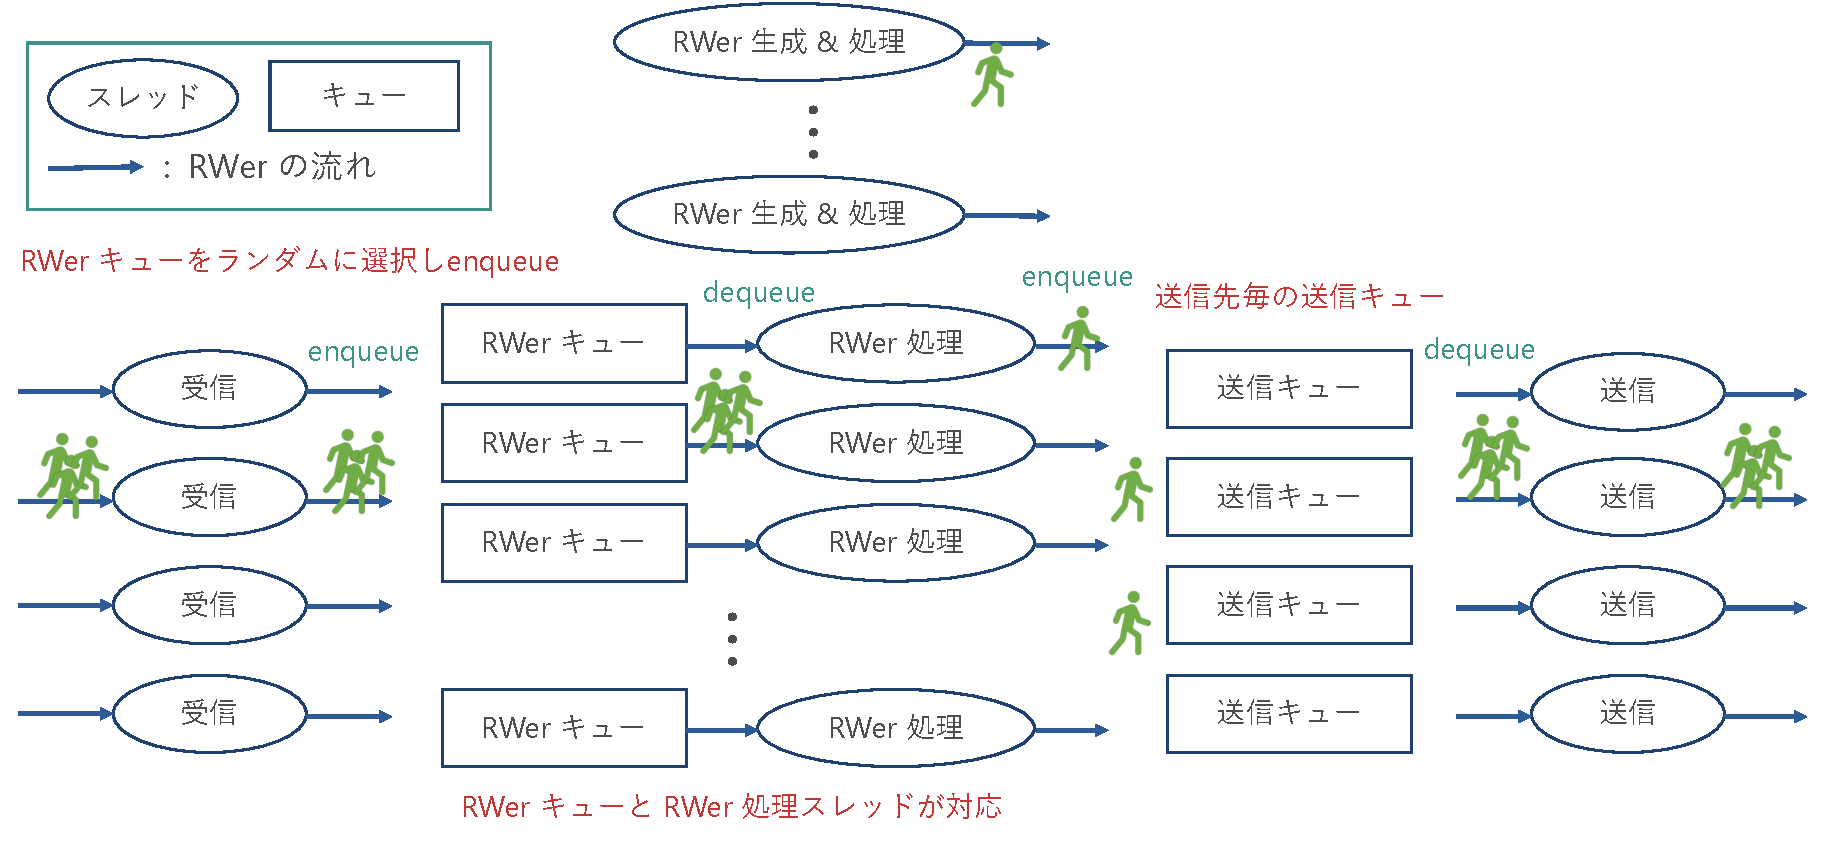
\includegraphics[scale=0.5]{figure/implementation.pdf}
    \caption{サーバ上の実装の概要.}
    \label{サーバ上の実装の概要}
\end{figure}

\section{終了した Random Walker の経路情報の保持方法}

\ref{Random Walker の経路再利用} で説明したように, 本手法では終了した RWer の経路情報を再利用することで通信のスキップを行う. そのためには終了した RWer の経路情報を保存しておく必要がある. 経路情報のまま保存するのは無駄が多いため, 経路再利用時に必要となる項目ごとに情報を保存する. 表 \ref{Random Walker の経路情報の保存形式} に RWer の経路情報の保存形式を示す. 本手法は C++ を使って実装しているためデータ構造は C++ の形式で記述した. 頂点に対する次数は RW 遷移時における index 選択の際に必要となる. データ構造に関しては, 頂点 ID を index とした配列の形で保持する. 頂点に対する持ち主サーバは, もし次の遷移先情報を持っていない場合に現在頂点の持ち主サーバへの RWer の送信が発生するため, 必要である. データ構造に関しては次数情報と同様, 頂点 ID を index とした配列の形で保持する. エッジデータは index を使った RW 遷移に必要となる. 例えば図 \ref{経路再利用による送信スキップ} ではサーバ 1 が (10, 0, 4), (10, 3, 11) (始点頂点, index, 遷移先頂点) というエッジデータを保持しているため, index = 0, 3 の場合は通信をスキップすることができる. データ構造に関しては, 頂点 ID を index とし, それぞれの頂点について (key, value) = (index, 遷移先頂点) のハッシュ map を保持する形とした. 

\begin{table}[t]
    \caption{Random Walker の経路情報の保存形式.}
    \label{Random Walker の経路情報の保存形式}
    \centering
    \begin{tabular}{cc}
        \hline
        保存項目  &  データ構造 (C++)  \\
        \hline \hline
        頂点に対する次数  &  std::vector$\langle$uint64$\_$t$\rangle$ \\
        \hline
        頂点に対する持ち主サーバ  &  std::vector$\langle$uint64$\_$t$\rangle$  \\
        \hline
        エッジデータ  &  std::vector$\langle$std::unordered$\_$map$\langle$uint64$\_$t, uint64$\_$t$\rangle$$\rangle$ \\
        \hline
    \end{tabular}
\end{table}

\section{受信スレッド}

\begin{algorithm}[t]
\DontPrintSemicolon
\nl $message \leftarrow$ 受信データ\;
\nl $message\_id \leftarrow message$ の先頭から抜き出した値\;
\nl \If{$message\_id ==$ 複数の RWer によるメッセージ} {
\nl     $RWer\_count \leftarrow message$ の先頭から抜き出した値\;
\nl     $RWer \;\; A[RWer\_count]$\;
\nl     $idx \leftarrow message$ 内における先頭の RWer 情報の開始位置\;
\nl     \For{$i = 1$ to $RWer\_count$} {
\nl         $A[i] \leftarrow message 内における i$ 個目の RWer の情報\;
\nl         $idx \leftarrow idx$ + ($i$ 個目の RWer のメモリサイズ)\;}
\nl     RWer キューをランダムに選択し, $A$ 内の RWer を全て格納\;}
\nl \Else{
\nl     他の場合は説明省略\;}
\caption{{受信スレッド} \label{受信スレッド}}
\end{algorithm}

\begin{table}[t!]
    \caption{メッセージの構成.}
    \label{メッセージの構成}
    \centering
    \begin{tabular}{ccc}
        \hline
        名称  &  サイズ  &  内容 \\
        \hline \hline
        $ver\_id\_$  &  8 bit  &  バージョン: 4 bit, メッセージ ID: 4 bit \\
        \hline
        $RWer\_count$  &  16 bit  &  メッセージ内に含まれる RWer の数 \\
        \hline
        複数の RWer  &  可変長サイズ $\times$ $RWer\_count$  &  表 \ref{RWer の構成} の RWer の情報を複数格納 \\
        \hline
    \end{tabular}
\end{table}

受信スレッドでは, 他のサーバから受信したメッセージを処理し, 適宜 RWer を RWer キューに格納する. メッセージの種類は複数の RWer 以外にも実験開始の合図, 結果送信の合図等があるが, ここでは主要な処理である複数の RWer について説明する. Algorithm \ref{受信スレッド} に受信スレッドの擬似コードを示す. また, 提案手法におけるメッセージ構成を表 \ref{メッセージの構成} に示す. まず, 受信したメッセージを $message$ に格納し, $message\_id$ を先頭の $ver\_id\_$ から抽出する (1, 2 行目). 次に $message$ からメッセージ内の RWer の個数である $RWer\_count$ を抽出し, サイズ $RWer\_count$ の RWer 格納用配列を作成する (4, 5 行目). そしてその配列 $A$ に $message$ 内の RWer の情報を格納していく(6 -- 9 行目). $idx$ は $message$ 内におけるそれぞれの RWer の情報の開始位置を表す. つまり, 6 行目において $idx$ = 24 bit であり, RWer の情報の開始位置は先頭から 25 bit 目である. RWer の情報は可変長なので, 2 つ目以降の RWer に関する $idx$ については, その都度一つ前の RWer のメモリサイズを表 \ref{RWer の構成} の $RWer\_size$ から読み取り, 加算する(9 行目). 最後に, 格納先の RWer キューをランダムに一つ選択し, $A$ 内の RWer を全て格納する(10 行目). 本手法では, 並列性を可能な限り保つことができる構築を意識しており, 受信スレッドごとに異なるポート番号を振り分け, 受信処理を並列に行う. また, RWer 処理スレッドも同様で, 図 \ref{サーバ上の実装の概要} のように各 RWer スレッドごとに RWer キューを用意した. 10 行目における RWer キューのランダム選択は, 各 RWer 処理スレッドの負荷分散のためである. また, $A$ 内の RWer それぞれに対してランダムな RWer キューを選択するのではなく, $A$ 内の全ての RWer をまとめて一つの RWer キューに格納するのは, RWer キューにて必要となる排他制御のロックを低減させるためである. 

本手法ではスレッド間での情報のやり取りが多い. 例えば, 受信スレッドと RWer 処理スレッド間では RWer キューを通じて RWer を受け渡す. ここでもし RWer を構造体のまま RWer キューへ push, または RWer キューから pull しようとすると, その都度構造体のメモリコピーが発生してしまいオーバヘッドが大きくなる. そのため本手法では情報の受け渡しをポインタで行う. また, スレッド間でのポインタの受け渡しには所有権の概念が存在するため, C++ におけるスマートポインタを利用してこの処理を実装した. 



\section{RWer 処理スレッド}

RWer 処理スレッドでは, RWer キューから RWer をまとめて取り出し, それぞれの RWer に対して RW 処理を行い, 他のサーバが所有する頂点への遷移が発生した場合は, その RWer を送信キューに格納する. Algorithm \ref{RWer 処理スレッド} に RWer 処理スレッドの擬似コードを示す. まず RWer キューから RWer をまとめて取り出し, 配列 $A$ に格納する(1, 2 行目). そして $A$ 内の各 $RWer$ について RW 処理を行う(3 -- 38 行目). RW 処理については, まず $RWer$ の $ver\_id\_$ (表 \ref{RWer の構成} 参照) から $message\_id$ を抽出し, それがもし終了した RWer のものだった場合, 終了した RWer に対する処理を行う(4 -- 6 行目). 終了した RWer に対する処理では主にその RWer の生成サーバに対応する送信キューへの push を行う. $message\_id$ が, まだ生存している RWer のものであった場合は, その RWer が終了 or 他のサーバが所有する頂点へ遷移し, 送信キューに格納されるまで処理を繰り返し行う(7 -- 38 行目). ここでの処理は $RWer$ の現在頂点である $current\_node$ (9 行目)が自サーバの所有頂点である場合とそうでない場合で異なる. $current\_node$ が自サーバの所有頂点である場合は, 基本的には自分が所持するグラフ上でのランダム遷移を行う. しかし 1 hop 前で通信が発生した, かつ $RWer$ の $next\_index\_$ (表 \ref{RWer の構成} 参照) に index 情報が格納されている場合は, 次の遷移はその index 情報を利用して行う(11 -- 14 行目). これは図 \ref{経路再利用による送信スキップ} の送信が発生したときのサーバ 2 上での処理に対応している. 遷移先 index のランダム選択は送信前に済ませているため, 送信先で再びランダム選択を行うと不正確な RW 遷移となってしまう. $current\_node$ が自サーバの所有頂点でない場合は, 過去の RWer の経路情報を利用して RW 遷移を行う. 22 行目における, 過去の経路情報から $current\_node$ の次数がわからない場合は, $current\_node$ が, 自分が所有する頂点の隣接頂点のうち, 他サーバが所有するかつまだ経路情報に含まれていない頂点であることがわかる. 本手法が想定する分散グラフ管理下では, 隣接頂点が他サーバの所有する頂点である場合, 自サーバはその頂点の ID と持ち主サーバの情報のみを保持するとしているため, $current\_node$ が自サーバの所有頂点でない (他サーバの頂点 ID 情報を持っている) かつ $current\_node$ の次数情報を持っていないという状態が存在する場合がある. このときは, $RWer$ を $current\_node$ の持ち主サーバへの送信キューへ push する(22, 23 行目). ここでは次数がわからず, index のランダム選択は行わない($RWer$ の $next\_index\_$ に値を入れない)ため, この $RWer$ を受信したサーバは, 11 行目における if 文を通過し, 通常のランダム遷移を行う. $current\_node$ の次数 ($degree$) が過去の経路情報からわかる場合, $degree$ 未満のランダムな値を $next\_index$ として, $current\_node$ の $next\_index$ 番目の隣接頂点を次の遷移先頂点 ($next\_node$) とする(26, 31, 32 行目). ここで, $next\_node$ が過去の経路情報から得られなかった場合は, $RWer$ の $next\_index\_$ に $next\_index$ を入れ, $current\_node$ の持ち主サーバへの送信キューへ push する(33 -- 35 行目). これは図 \ref{経路再利用による送信スキップ} において, サーバ 1 上で 1 or 2 の index を選択した場合に対応する. この RWer を受信したサーバは, 11 行目の if 分で引っかかり, index 情報による決定的な遷移を行う. $next\_node$ が過去の経路情報から得られた場合は, $RWer$ をその $next\_node$ に遷移させる(38 行目). 
\\
\\
\\
\\

\begin{algorithm}[p]
\DontPrintSemicolon
\nl vector$\langle$RWer$\rangle$ $\; A$\;
\nl $A \leftarrow$ RWer キューから RWer をまとめて取り出し, 格納\;
\nl \For{$each \; RWer \in A$} {
\nl     $message\_id \leftarrow RWer$ の $ver\_id\_$ から抽出\;
\nl     \If{$message\_id ==$ 終了した RWer} {
\nl         終了した RWer に対する処理\;}
\nl     \ElseIf{$message\_id ==$ 生存している RWer} {
\nl         \While{true} {
\nl             $current\_node \leftarrow RWer$ の現在頂点\;
\nl             \If{$current\_node$ が自サーバの所有頂点である場合} {
\nl                 \If{1 hop 前で通信が発生した $\&\&$ 次の遷移先の index 情報が格納されている} {
\nl                     $next\_index \leftarrow RWer の next\_index\_$\;
\nl                     $next\_node \leftarrow$ $current\_node$ の隣接リストの $next\_index$ 番目の頂点\;
\nl                     $RWer$ を $next\_node$ に遷移させる\;}
\nl                 \ElseIf{$RWer$ の $RWer\_life\_$ が 0 \textbar\textbar $\;current\_node$ の次数が 0} {
\nl                     終了した RWer に対する処理\;
\nl                     break\;}
\nl                 \Else {
\nl                     $next\_node \leftarrow$ $current\_node$ のランダムな隣接頂点\;
\nl                     $RWer$ を $next\_node$ に遷移させる\;}}
\nl             \ElseIf{$current\_node$ が自サーバの所有頂点でない場合} {
\nl                 \If{過去の経路情報から $current\_node$ の次数情報がわからない場合} {
\nl                     $current\_node$ の持ち主サーバへの送信キューに $RWer$ を push\;
\nl                     break\;}
\nl                 \Else {
\nl                     $degree \leftarrow$ 過去の経路情報から得られた $current\_node$ の次数\;
\nl                     \If{$RWer$ の $RWer\_life\_$ が 0 \textbar\textbar $\;degree == 0$} {
\nl                         終了した RWer に対する処理\;
\nl                         break\;}
\nl                     \Else {
\nl                         $next\_index \leftarrow 0 \leq r < degree$ のランダムな値 $r$\;
\nl                         $next\_node \leftarrow current\_node$ の $next\_index$ 番目の隣接頂点\;
\nl                         \If{$next\_node$ が過去の経路情報から得られなかった場合} {
\nl                             $RWer$ の $next\_index\_ \leftarrow next\_index$\;
\nl                             $current\_node$ の持ち主サーバへの送信キューに $RWer$ を push\;
\nl                             break\;}
\nl                         \Else {
\nl                             $RWer$ を $next\_node$ に遷移させる\;}}}}}}}
\caption{{RWer 処理スレッド} \label{RWer 処理スレッド}}
\end{algorithm}

\section{送信スレッド}\label{sub:送信スレッド}

送信スレッドでは, 送信先ごとの送信キューから RWer をまとめて取り出し, メッセージを生成し,他サーバへ送信する. Algorithm \ref{送信スレッド} に送信スレッドの擬似コードを示す. 1 -- 3 行目は各送信スレッドがどの送信キューを選択するかを決める処理を表している. 本手法では送信キューが送信先ごとに生成されるのに対し送信スレッド数は最初から決まっているため, それぞれの送信スレッドはどの送信キューに格納されている RWer を送信するのかを決める必要がある. 送信スレッド間で同時に同じ送信キューが選択されることを防ぐため, 1 -- 3 行目は送信スレッド間での排他制御となっている. $id\_num\_$ は全送信スレッド間での共有変数であり, 暫定送信先 ID を示す. この $id\_num\_$ が自サーバのものでないかつ, 他のサーバが $id\_num\_$ 番目の送信キューを占有していない状態を満たすまで $id\_num\_$ をインクリメントする(1 -- 2 行目). 条件を満たす $id\_num\_$ が得られたらスレッド内変数である $send\_id$ に格納する(3 行目). その後, $send\_id$ 番目の送信キューから RWer をまとめて取り出し, 配列 $A$ に格納する. 6 行目以降は配列 $A$ 内の $RWer$ をできるだけまとめながら送信する処理を表している. $message$ は送信するメッセージを入れる変数, $RWer\_count$ は一つのメッセージ内に含まれる RWer の数, $now\_message\_size$ は現在のメッセージサイズを示しており(6 -- 8 行目), メッセージサイズの初期値は $ver\_id\_$ と $RWer\_count$ のサイズの合計である 24 となる (表 \ref{メッセージの構成}). 9 -- 20 行目の for 文ではメッセージに $RWer$ のデータを書き込んでいくが, その際メッセージサイズが指定された最大サイズを超えてしまう場合はデータ書き込みの前にメッセージ送信を行う. 送信時のポート番号については受信ポート番号からランダムに一つ選択し, 設定する. メッセージ送信後は $message$, $RWer\_count$, $now\_message\_size$ を初期値に戻す. 全ての $RWer$ のメッセージへの書き込みが終わった後, メッセージ内に $RWer$ が残っていた場合はその $message$ を送信する(21, 22 行目). 送信におけるメッセージの最大サイズについては, MTU - IP ヘッダ (20 byte) - UDP ヘッダ (8 byte) とする. 送信データサイズが MTU を超えるとパケット分割が発生し, パケットロス時の RWer 損失数が増えてしまうためである. 実験においては MTU を 9000 に設定しているため, 送信スレッドにおけるメッセージの最大サイズは 8972 byte となる. 

\begin{algorithm}[t!]
\DontPrintSemicolon
\nl \While{$id\_num\_ == hostid\_ \;$ \textbar\textbar 他のサーバが $id\_num\_$ 番目の送信キューを占有している} {
\nl     $id\_num\_ \leftarrow (id\_num\_ + 1)\; \%$ 送信キューの数\;}
\nl $send\_id \leftarrow id\_num\_$\;
\nl vector$\langle$RWer$\rangle$ $\; A$\;
\nl $A \leftarrow send\_id$ 番目の送信キューから RWer をまとめて取り出し, 格納\;
\nl $message \leftarrow$ 空のメッセージ\;
\nl $RWer\_count \leftarrow 0$\;
\nl $now\_message\_size \leftarrow $ sizeof($ver\_id\_$) + sizeof($RWer\_count$)\;
\nl \For{$each \; RWer \in A$} {
\nl     $RWer\_size \leftarrow RWer$ のメモリサイズ\;
\nl     \If{$now\_message\_size + RWer\_size \geq $ メッセージの最大サイズ} {
\nl         $message$ に $ver\_id\_$ と $RWer\_count$ を格納\;
\nl         $port\_num \leftarrow$ 指定されたポート番号の中からランダム選択\;
\nl         $message$ を $send\_id$ の送信先へ送信 (ポート番号は $port\_num$)\;
\nl         $message \leftarrow$ 空のメッセージ\;
\nl         $RWer\_count \leftarrow 0$\;
\nl         $now\_message\_size \leftarrow $ sizeof($ver\_id\_$) + sizeof($RWer\_count$)\;}
\nl     $RWer$ を $message$ に書き込む\;
\nl     $RWer\_count \leftarrow RWer\_count + 1$\;
\nl     $now\_message\_size \leftarrow now\_message\_size + RWer\_size$\;}
\nl \If{$RWer\_count > 0$} {
\nl     残った $message$ を上記と同様にして送信\;}
\caption{{送信スレッド} \label{送信スレッド}}
\end{algorithm}

\chapter{評価}
\label{chap:eval}
\section{目的}
本研究では, 地理的分散環境下における分散グラフ RW 実行エンジンを提案した. 提案手法を既存の分散グラフ RW 実行エンジンである KnightKing \cite{10.1145/3341301.3359634} と比較することで, 地理的分散環境下における本手法の有用性を明らかにする. また, 送信時に RWer をまとめることによる性能向上の評価, そして経路再利用のための再利用エッジデータが貯まるまでの RW 実行数の評価を行うことで, 本手法の構成要素に関する検討も行った. 

\section{項目}

評価項目は以下の通りである. 
\begin{quote}
    \begin{itemize}
        \item 既存手法との比較
        \begin{itemize}
            \item RTT, パケットロス率を変えた場合の実行時間
            \item Random Walker の経路再利用をした場合の実行時間
            \item グラフ分割の汚さを変えた場合の実行時間
            \item グラフ分割数 (サーバ台数) を変えた場合の実行時間
            \item Random Walk の終了確率 $\alpha$ を変えた場合の実行時間
        \end{itemize}
        \item 提案手法に関する検討
        \begin{itemize}
            \item Random Walker をまとめて送信したことによる速度向上
            \item 再利用エッジが貯まるまでに実行する Random Walk の回数
        \end{itemize}
    \end{itemize}
\end{quote}

\section{評価環境}

\subsection{データセット}

本評価では実世界グラフと生成グラフの両方を使用して実験を行った. 実世界グラフは LiveJournal のデータセット\cite{snapnets} (頂点数 3,997,962, 辺数 69,362,378) を使用した. 生成グラフに関しては, エッジ生成確率を制御できるアルゴリズムである, Stochastic block model (SBM) \cite{SBM} を使用した. SBM では, partition 数, 各 partition 内の頂点数, partition 内の頂点間のエッジ生成確率, partition 間の頂点間のエッジ生成確率を指定し, グラフを生成することができる. このエッジ生成確率を操作することで, 例えばサーバ間を跨ぐ RW 遷移が多くなるグラフを生成することができる. 生成グラフの頂点数とエッジ生成確率の値に関しては, 実験 \ref{グラフ分割の汚さを変えた場合の実行時間}, \ref{グラフ分割数を変えた場合の実行時間} で説明する. 

\subsection{評価環境}

本評価では最大 7 台のサーバを使用して実験を行った. 各サーバは全て同じ性能をしており, 表 \ref{評価環境} に示す. また, 実装は全て C++ で行った. 

\begin{table}[t]
    \caption{評価環境.}
    \label{評価環境}
    \centering
    \begin{tabular}{c|c}
      \hline
      項目 & 内容   \\
      \hline \hline
      OS  & Ubuntu 20.04 LTS \\
      CPU  & Intel(R) Xeon(R) CPU E5-2643 v2 @ 3.50GHz  \\
      Core & 24 (hyper threading 有効) \\
      RAM  & 32GB \\
      \hline
    \end{tabular}
\end{table}

\subsection{RW 実行について}

本評価における RW 実行のに実行時間について, 開始時間は RWer を生成し始めるタイミングで, 終了時間は全てのサーバで全ての RWer の終了確認が取れたタイミングとしている. 既存手法と異なり提案手法は UDP 通信を使用しているため, パケットロスによる RWer の損失が発生する. 本来提案手法では, RWer の損失の影響が少ない (図 \ref{局所的に RWer が損失したときの PPR 演算の精度} 参照) ことを理由にパケットロスを許容しているが, 全ての RWer の終了を前提としている既存手法との比較のために, 簡易的な再送機能を実装した. 再送スレッドは全体の 95 \% の RW 実行が終了した時点で起動し, 3 秒ごとにまだ終了確認の取れてない RWer を再生成する.  

\section{既存手法との比較}

\subsection{RTT, パケットロス率を変えた場合の実行時間}\label{RTT, パケットロス率を変えた場合の実行時間}

\begin{figure}[t]
    \centering
    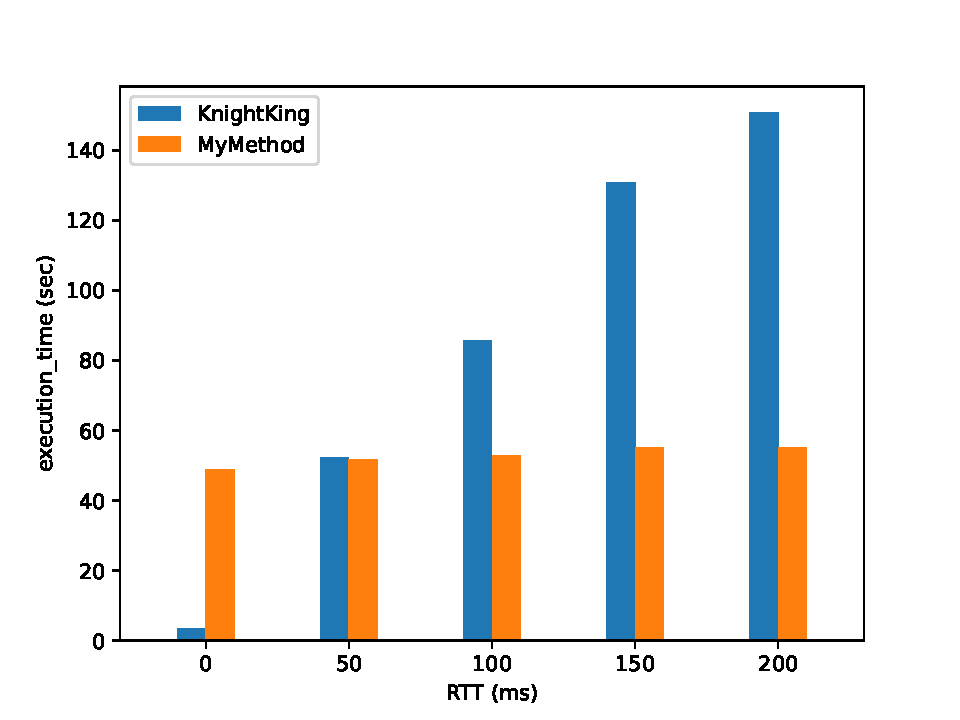
\includegraphics[scale=0.8]{figure/Kn_vs_AR_RTT.pdf}
    \caption{パケットロス率を 0.03 \% に固定したときの実行時間.}
    \label{パケットロス率を 0.03 に固定したときの実行時間}
\end{figure}

\begin{figure}[t!]
    \centering
    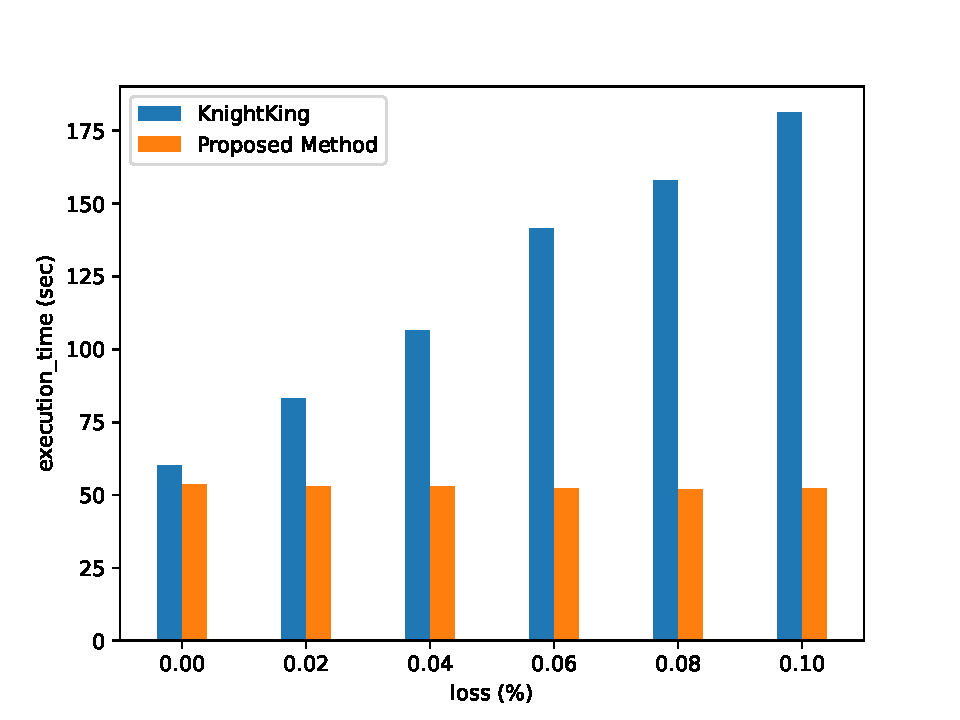
\includegraphics[scale=0.8]{figure/Kn_vs_AR_loss.pdf}
    \caption{RTT を 100 ms に固定したときの実行時間.}
    \label{RTT を 100 ms に固定したときの実行時間}
\end{figure}

データセットは実世界グラフ, サーバ数は 5 台で実験を行った. まず, 実験前にグラフを 5 分割し, 各サーバに配置する. ここでの分割方法はハッシュ分割 (ランダム分割) である. 具体的には, 各サーバの ID を 0 $\sim$ 4 とし, 各頂点をサーバ ID = 頂点 ID \% 5 のサーバに配置する. この先特に指定がない場合は, 分割に関してはこのハッシュ分割を採用している. そして RW 実行に関しては, 終了確率 $\alpha$ = 0.15 の RW を各頂点から 10 回ずつ実行する. 実世界グラフの頂点数は 3,997,962 なので実行する RW 数は合計 39,979,620 回となる. 実験結果を図 \ref{パケットロス率を 0.03 に固定したときの実行時間}, \ref{RTT を 100 ms に固定したときの実行時間} に示す. まず, 図 \ref{パケットロス率を 0.03 に固定したときの実行時間} は, サーバ間のパケットロス率を 0.03 \% に固定し, RTT を 0 $\sim$ 200 ms で変動させて実験を行った結果である. 既存手法では RTT が 0 ms, 50 ms, 100 ms, 150 ms, 200 ms と変化すると実行時間が約 4 秒, 52 秒, 86 秒, 131 秒, 151 秒となり, 大幅に増加していることがわかる. これは既存手法が TCP 通信を使用していることが原因であり, RTT が大きくなるとスループットが小さくなる. 対して提案手法では RTT が 0 ms, 50 ms, 100 ms, 150 ms, 200 ms と変化すると実行時間が約 49 秒, 52 秒, 53 秒, 55 秒, 55 秒となっており, 既存手法と比べてあまり増加しないことがわかる. これは提案手法が UDP 通信を使用しているためであり, RTT が変化してもスループットの変化は小さい. RTT が 0 のときは既存手法が 4 秒, 提案手法が 49 秒と既存手法の方が約 12 倍高速である. これは, 既存手法における RWer の送信では経路情報を送らないため通信量が少ないこと, そして同期処理によって CPU リソースを最大限活用することができていることが要因であると考える. 図 \ref{RTT を 100 ms に固定したときの実行時間} は, サーバ間の RTT を 100 ms に固定し, パケットロス率を 0 $\sim$ 0.1 \% で変動させて実験を行った結果である. こちらも 図 \ref{パケットロス率を 0.03 に固定したときの実行時間} と同様に, パケットロス率の増加とともに実行時間が大きく増加する既存手法に対し, 提案手法では実行時間がほとんど変化していない. これらの結果から, RTT, パケットロス率が無視できるような環境では既存手法のような TCP 通信を使った同期処理による RW 処理, 地理的分散環境のような RTT, パケットロス率が無視できない環境では提案手法のような UDP 通信を使った非同期処理が適していることがわかる. 

\subsection{Random Walker の経路再利用をした場合の実行時間}\label{Random Walker の経路再利用をした場合の実行時間}

データセットは実世界グラフ, サーバ数は 5 台で実験を行った. RW 実行に関しては \ref{RTT, パケットロス率を変えた場合の実行時間} と同様で, 終了確率 $\alpha$ = 0.15 の RW を各頂点から 10 回ずつ実行する. また, RTT は 100 ms, パケットロス率は 0.03 \% でそれぞれ固定し, 再利用するためのエッジデータは実験前に調達済みであるとする. 図 \ref{経路再利用をしたときの実行時間} に経路再利用をしたときの実験結果を示す. 緑の点線は既存手法を, 青い棒は提案手法の経路再利用をしないもの, オレンジ色の棒は提案手法の経路再利用をするものを表す. 横軸における original edges は元々各サーバが保持していたエッジの数であり, reuse edges は再利用エッジの数である. 実世界グラフにおけるエッジの数は全部で 69,362,378 なので, これを 5 分割した約 14,000,000 が original edges の値となる. つまり, original edges + reuse edges = 20,000,000 のとき, reuse edges の値は約 6,000,000 である. 実験結果について, 提案手法の経路再利用をしない場合は既存手法に比べて約 1.6 倍高速であり, 提案手法の経路再利用をする場合はそれぞれ提案手法に比べて約 2.2 倍, 2.9 倍, 3.8 倍, 5.0 倍, 7.2 倍高速だった. 結果から RWer の経路再利用により実行時間を削減できていることがわかる. また, 経路再利用による削減時間を再利用エッジ数で割ることにより, 再利用エッジ 1 本あたりの時間削減量を求めたところ, original edges + reuse edges ($\times$ 10000) = 2000, 3000, 4000, 5000, 6000 でそれぞれ約 0.024, 0.014, 0.012, 0.010, 0.009 になった. この結果から, 再利用エッジが増えれば増えるほど再利用エッジ 1 本あたりの時間削減量が減ることがわかった. 

\begin{figure}[t]
    \centering
    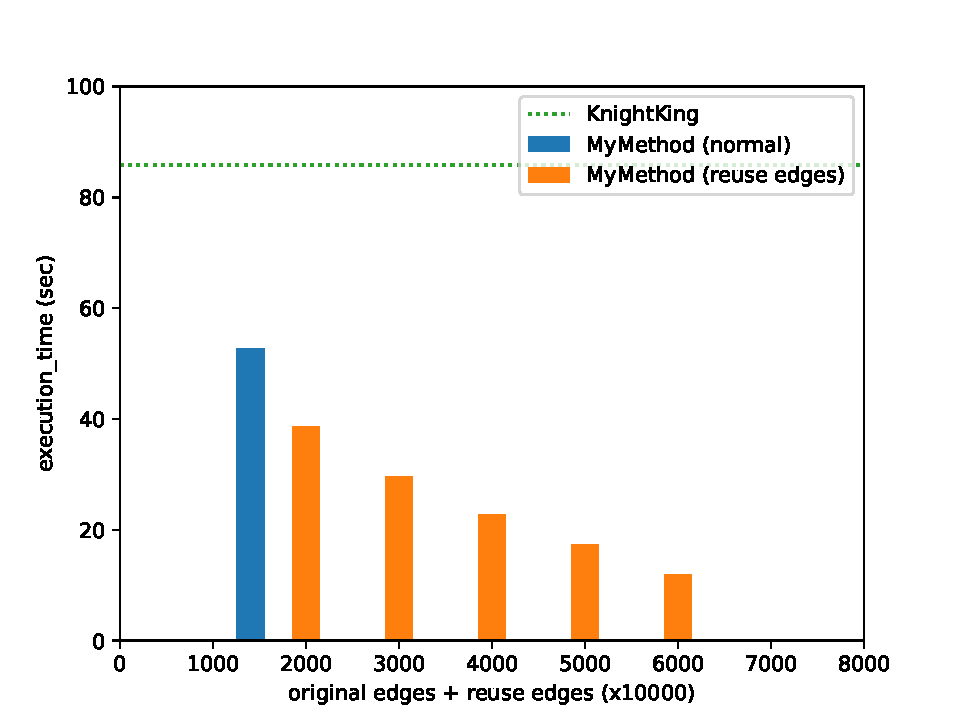
\includegraphics[scale=0.8]{figure/AR_cache.pdf}
    \caption{経路再利用をしたときの実行時間.}
    \label{経路再利用をしたときの実行時間}
\end{figure}

\subsection{グラフ分割の汚さを変えた場合の実行時間}\label{グラフ分割の汚さを変えた場合の実行時間}

\begin{figure}[t]
    \centering
    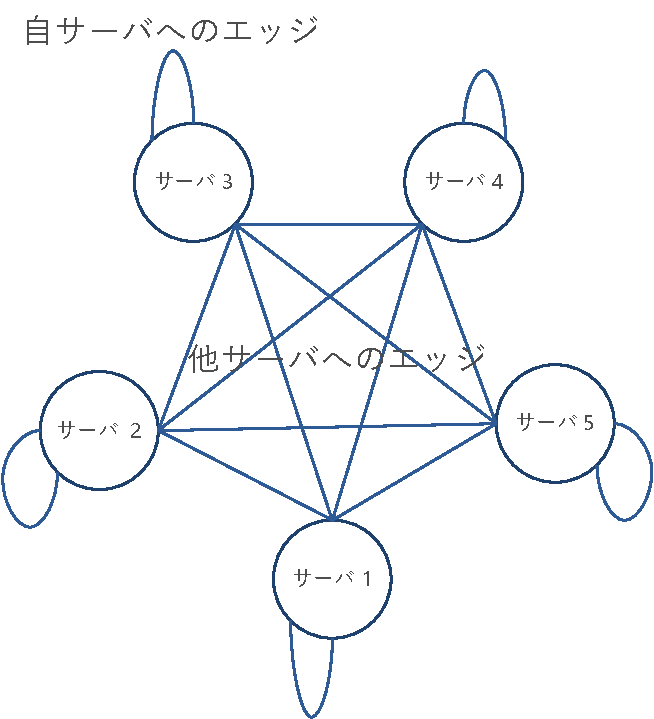
\includegraphics[scale=0.7]{figure/sbm.pdf}
    \caption{SBM による生成グラフの構造.}
    \label{SBM による生成グラフの構造}
\end{figure}

\begin{figure}[t!]
    \centering
    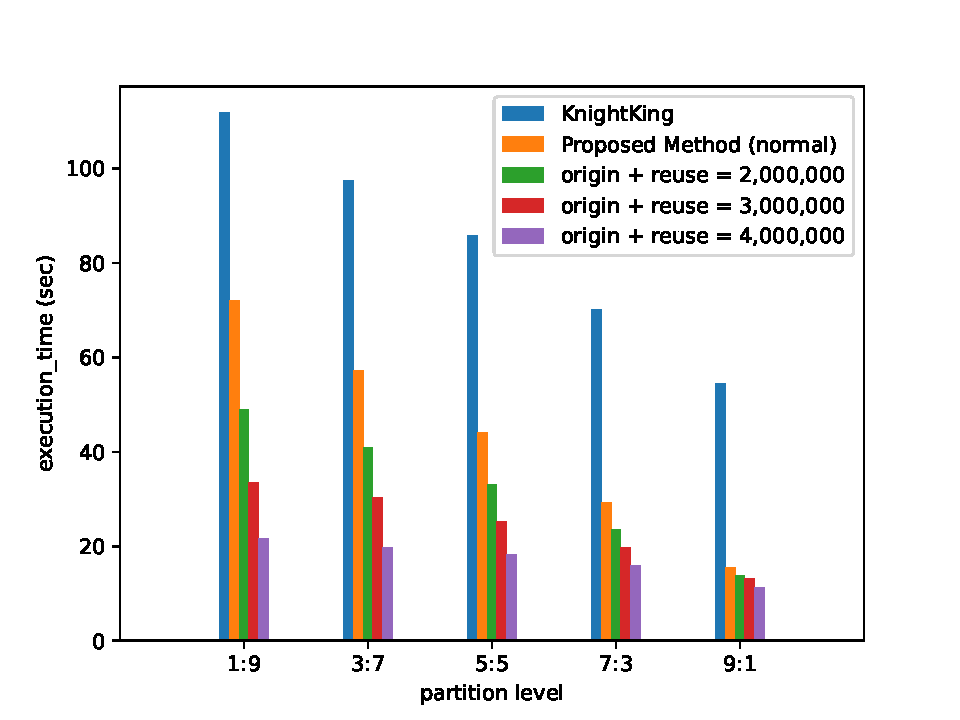
\includegraphics[scale=0.9]{figure/Kn_vs_AR_partition_level.pdf}
    \caption{グラフ分割の汚さを変えた場合の実行時間.}
    \label{グラフ分割の汚さを変えた場合の実行時間の結果}
\end{figure}

データセットは生成グラフ, サーバ台数は 5 台で実験を行った. 生成グラフは SBM で作成しており, 図 \ref{SBM による生成グラフの構造} に構造を示す. SBM における partition 数 は 5, 各 partition 内の頂点数は 10000 としたため, 全グラフでの頂点数は 50000 となる. そして, partition 内の頂点間のエッジ生成確率 (自サーバへのエッジ) と partition 間の頂点間のエッジ生成確率 (他サーバへのエッジ) の比率を操作することにより, グラフ分割の汚さを表現した. 例えば, 他サーバへのエッジの比率が自サーバへのエッジの比率よりも大きければ大きいほど, 他サーバが所有する頂点への RW 遷移が増えるため, サーバ間通信量が増える.  本実験においてはサーバ間通信が多くなるようなグラフ分割が汚いグラフ分割であるとする. 生成確率の値については, 各サーバでのエッジ数の期待値が 1,000,000 になるように設定した. 例えば, 自サーバへのエッジ数 : 他サーバへのエッジ数 = 1 : 9 とする場合は, partition 内の頂点間のエッジ生成確率 = 0.1 \%, partition 間の頂点間のエッジ生成確率 = 0.225 \% とすることで, 自サーバへのエッジ数の期待値が 100,000, 他サーバへのエッジ数の期待値が 900,000 となり, 合計のエッジ数の期待値が 1,000,000 となる. また, サーバ数 は 5 なので, 全グラフでのエッジ数は 5,000,000 である. RW 実行に関しては, 終了確率 $\alpha$ = 0.15 の RW を各頂点から 1000 回ずつ実行する. 生成グラフの頂点数は 50000 なので実行する RW 数は合計 50,000,000 回となる. また, RTT は 100 ms, パケットロス率は 0.03 \% でそれぞれ固定し, 再利用するためのエッジデータは実験前に調達済みであるとする. 図 \ref{グラフ分割の汚さを変えた場合の実行時間の結果} に実験結果を示す. 横軸は自サーバへのエッジ数 : 他サーバへのエッジ数を表しており, 左に行くにつれ汚い分割になる. 横軸が 1 : 9 のとき, 提案手法は既存手法に比べてそれぞれ約 1.6 倍, 2.3 倍, 3.3 倍, 5.1 倍高速になり, 横軸が 7 : 3 のとき, 提案手法は既存手法に比べてそれぞれ約 2.4 倍, 3.0 倍, 3.5 倍, 4.4 倍高速になった. また, 提案手法における経路再利用の有無について, 横軸が 1 : 9 のとき, 経路再利用をする場合はしない場合に比べてそれぞれ約 1.47 倍, 2.15 倍, 3.32 倍高速になり, 横軸が 3 : 7 のとき, 経路再利用をする場合はしない場合に比べてそれぞれ約 1.24 倍, 1.48 倍, 1.84 倍高速になった. これらの結果から, 分割が汚ければ汚いほど, 提案手法における RWer の経路再利用の効果が大きくなるということがわかった. 地理的分散環境下では各地域ごとにグラフ編集が発生し, 全体で見たときの分割精度の制御ができないため, 分割が汚くなる場合が十分考えられるが, その場合でも提案手法は有効である. 

\subsection{グラフ分割数 (サーバ台数) を変えた場合の実行時間}\label{グラフ分割数を変えた場合の実行時間}

\begin{figure}[t]
    \centering
    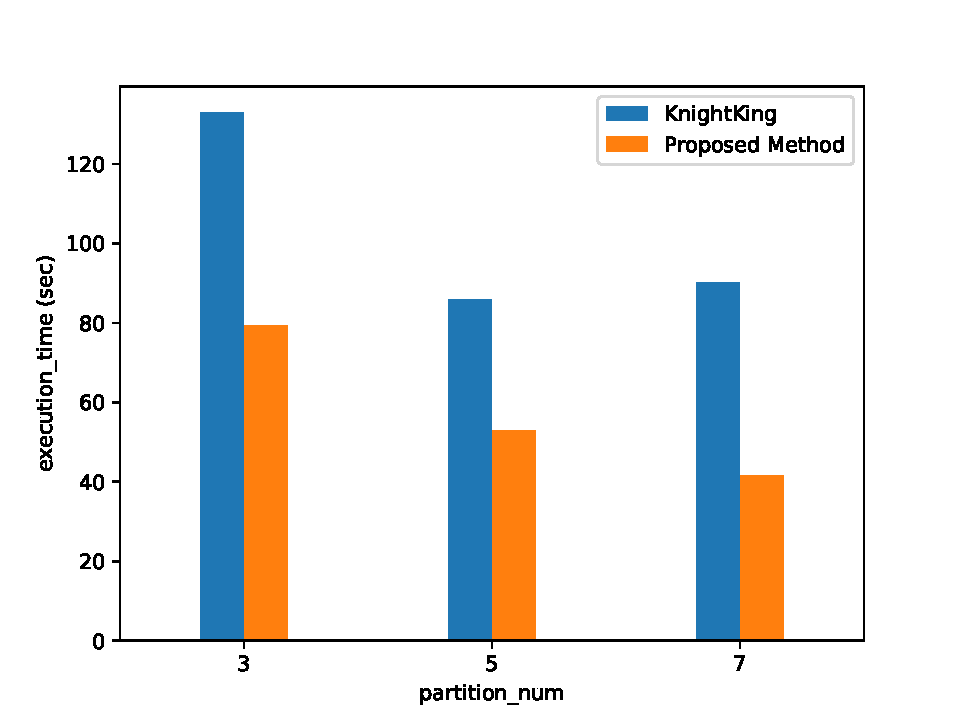
\includegraphics[scale=0.8]{figure/Kn_vs_AR_partition_num_LiveJournal.pdf}
    \caption{グラフ分割数を変えた場合の実行時間 (実世界グラフ).}
    \label{グラフ分割数を変えた場合の実行時間 (実世界グラフ)}
\end{figure}

\begin{figure}[t!]
    \centering
    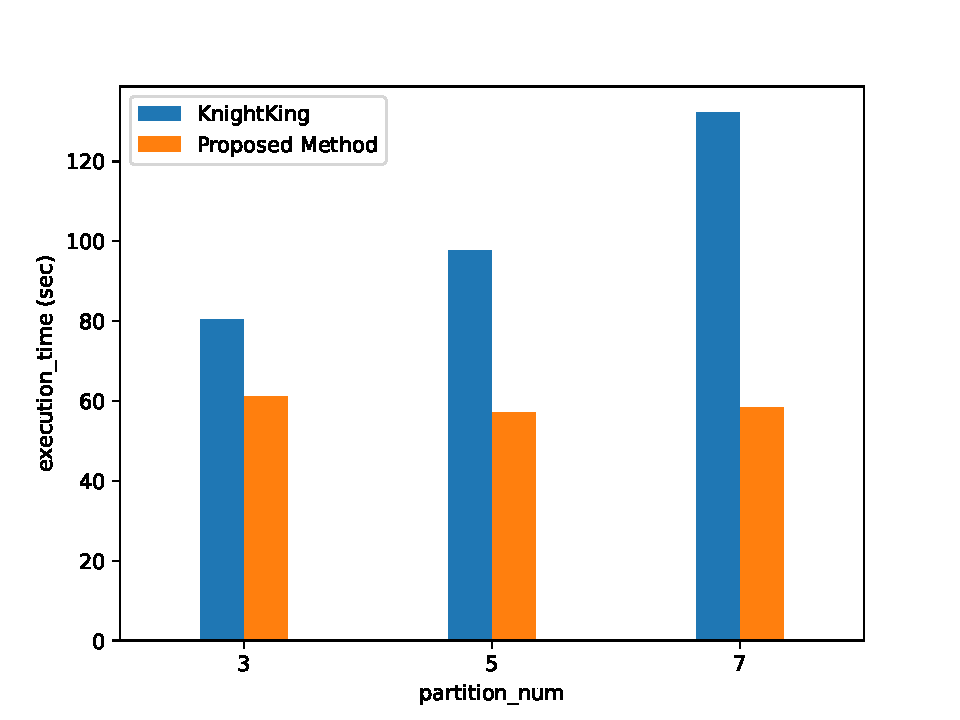
\includegraphics[scale=0.8]{figure/Kn_vs_AR_partition_num_SBM_3.pdf}
    \caption{グラフ分割数を変えた場合の実行時間 (生成グラフ).}
    \label{グラフ分割数を変えた場合の実行時間 (生成グラフ)}
\end{figure}

データセットは実世界グラフ, 生成グラフの両方を使用し, サーバ台数は 3, 5, 7 台で実験を行った. 経路の再利用は行っていない. 実世界グラフを使った実験ではサーバ台数に合わせてグラフの分割を行う. RW 実行に関しては終了確率 $\alpha$ = 0.15 の RW を各頂点から 10 回ずつ実行する. また, RTT は 100 ms, パケットロス率は 0.03 \% でそれぞれ固定した. 図 \ref{グラフ分割数を変えた場合の実行時間 (実世界グラフ)} に実験結果を示す. 既存手法では, 分割数が 3 から 5 に変化した場合約 1.55 倍高速になるが, 分割数が 5 から 7 に変化した場合は約 1.05 倍遅くなる. 提案手法では, 分割数が 3 から 5 に変化した場合約 1.50 倍高速になり, 分割数が 5 から 7 に変化した場合は約 1.27 倍高速になる. この結果から分割数(サーバ台数)が 5 から 7 に変化したとき, 計算資源 (サーバ台数) の増加による高速化と通信量 (分割数) 増加による低速化に注目すると, 既存手法では通信量 (分割数) 増加による低速化が上回り, 提案手法では計算資源 (サーバ台数) の増加による高速化が上回ることがわかる. 生成グラフを使った実験では, サーバ台数を変化させても 1 つのサーバあたりの頂点数, 辺数を変化させない (それぞれ 10000, 1,000,000) ようにグラフを生成した. つまり, サーバ台数が 3, 5, 7 と変化すると全グラフでの頂点数, 辺数は, (30000, 3,000,000), (50000, 5,000,000), (70000, 7,000,000) となる. このようにすることでシステム規模を拡大した状況を想定した実験を行うことができる. RW 実行に関しては終了確率 $\alpha$ = 0.15 の RW を各頂点から 1000 回ずつ実行する. RW 実行数の合計はサーバ台数が 3, 5, 7 と変化すると, 30,000,000, 50,000,000, 70,000,000 と変化する. 図 \ref{グラフ分割数を変えた場合の実行時間 (生成グラフ)} に実験結果を示す. 既存手法では, 分割数が 3 から 5 に変化した場合約 1.21 倍遅くなり, 分割数が 5 から 7 に変化した場合は約 1.35 倍遅くなる. 提案手法では, 分割数が 3 から 5 に変化した場合約 1.06 倍高速になり, 分割数が 5 から 7 に変化した場合は約 1.02 倍遅くなる. 実行時間に影響を及ぼすのは, 計算資源 (サーバ台数) の増加による高速化と RW 実行回数の増加と通信量増加による低速化であり, 既存手法では計算資源 (サーバ台数) の増加による高速化が上回る. 対して提案手法ではこれらがほとんど釣り合っており, 実行時間の変化が少ない. 以上の結果から提案手法は既存手法と比べシステム規模に対するスケーラビリティが高いことがわかった. 

\subsection{Random Walk の終了確率 $\alpha$ を変えた場合の実行時間}\label{終了確率 alpha を変えた場合の実行時間}

\begin{figure}[t]
    \centering
    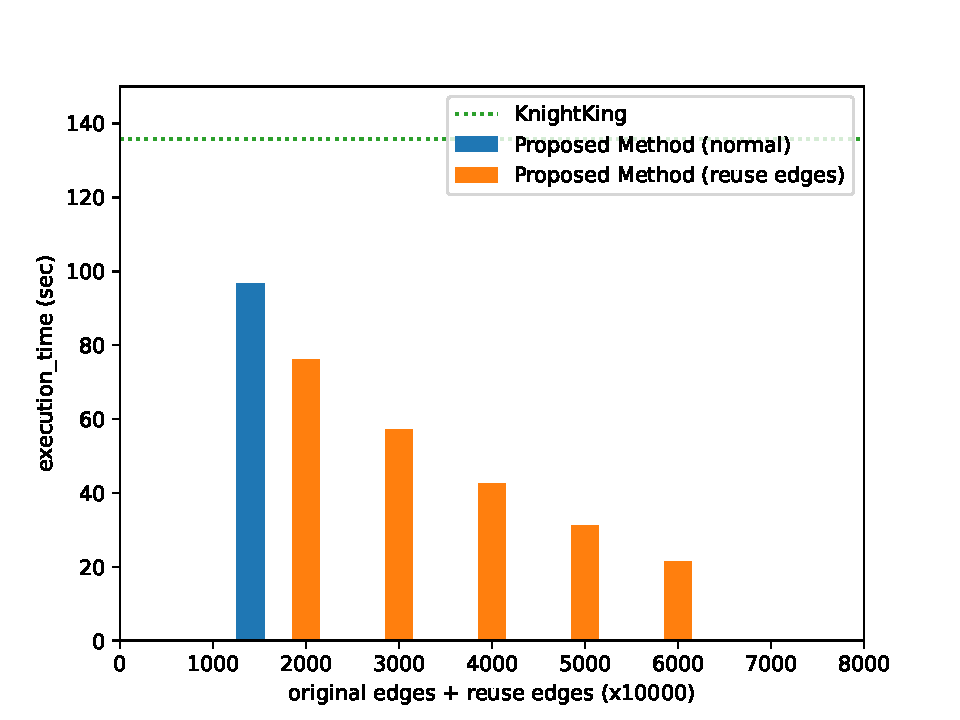
\includegraphics[scale=0.8]{figure/AR_cache_alpha_0.1.pdf}
    \caption{$\alpha$ = 0.1 のときの実行時間.}
    \label{alpha = 0.1 のときの実行時間}
\end{figure}

\begin{figure}[t!]
    \centering
    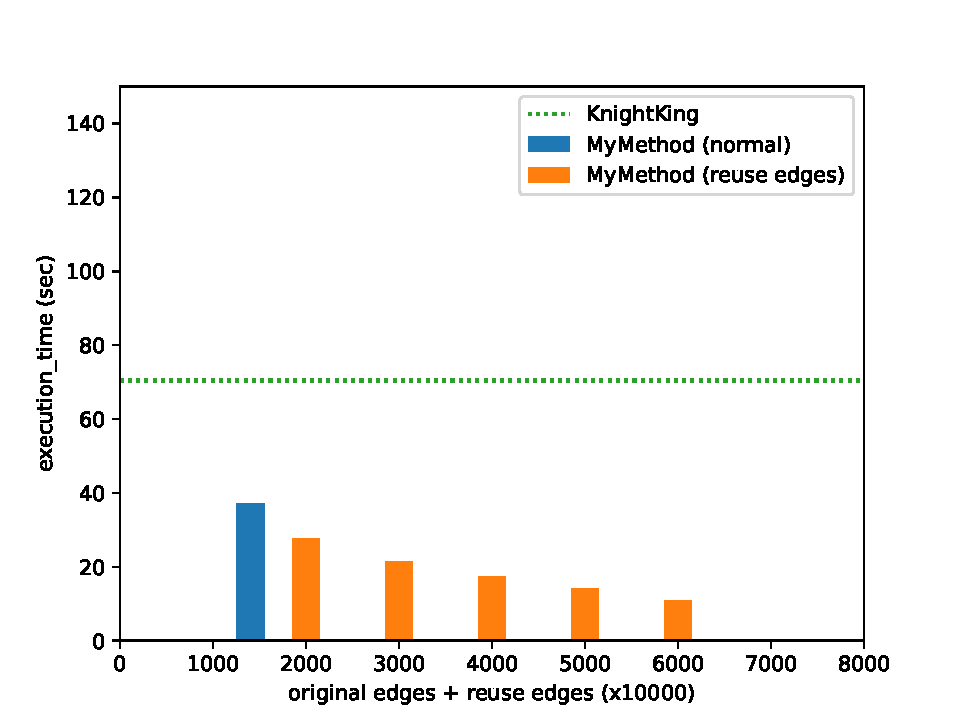
\includegraphics[scale=0.8]{figure/AR_cache_alpha_0.2.pdf}
    \caption{$\alpha$ = 0.2 のときの実行時間.}
    \label{alpha = 0.2 のときの実行時間}
\end{figure}

データセットは実世界グラフ, サーバ数は 5 台で実験を行った. RW 実行に関しては, 終了確率 $\alpha$ = 0.1, 0.2 の RW を各頂点から 10 回ずつ実行する. また, RTT は 100 ms, パケットロス率は 0.03 \% でそれぞれ固定した. 図 \ref{alpha = 0.1 のときの実行時間} に $\alpha$ = 0.1 のときの実行時間を, 図 \ref{alpha = 0.2 のときの実行時間} に $\alpha$ = 0.2 のときの実行時間を示す. $\alpha$ = 0.1 のとき, 提案手法は既存手法に比べてそれぞれ約 1.4 倍, 1.8 倍, 2.4 倍, 3.2 倍, 4.4 倍, 6.3 倍高速になり, $\alpha$ = 0.2 のとき, 提案手法は既存手法に比べてそれぞれ約 1.9 倍, 2.6 倍, 3.3 倍, 4.1 倍, 5.0 倍, 6.5 倍高速になった. また, 提案手法における経路再利用の有無について, $\alpha$ = 0.1 のとき, 経路再利用をする場合はしない場合に比べてそれぞれ約 1.27 倍, 1.69 倍, 2.27 倍, 3.10 倍, 4.52 倍高速になり, $\alpha$ = 0.2 のとき, 経路再利用をする場合はしない場合に比べてそれぞれ約 1.35 倍, 1.73 倍, 2.14 倍, 2.62 倍, 3.42 倍高速になった. これらの結果から, 再利用エッジが増えていくと, $\alpha$ = 0.2 のときよりも $\alpha$ = 0.1 のときの方が経路再利用効果が大きくなることがわかる. これは $\alpha$ = 0.1 の方が RW の経路長の期待値が大きい(通信量が増える)ため, 経路再利用による通信スキップの恩恵が大きくなるからであると考える.

\section{提案手法に関する検討}

\subsection{Random Walker をまとめて送信したことによる速度向上}\label{Random Walker をまとめて送信した場合とそうでない場合の実行時間}

データセットは実世界グラフ, サーバ数は 5 台で実験を行った. RW 実行に関しては, 終了確率 $\alpha$ = 0.15 の RW を各頂点から 10 回ずつ実行する. また, RTT は 100 ms, パケットロス率は 0.03 \% でそれぞれ固定した. 本実験では RWer 単体で送信する場合と複数の RWer をまとめて送信する場合の提案手法における実行時間の比較をした. 具体的には, 複数の RWer をまとめて送信する場合は \ref{sub:送信スレッド} で説明した方法で送信し, RWer 単体での送信では表 \ref{メッセージの構成} の $RWer\_count$ を必ず 1 にして送信を行う. 図 \ref{Random Walker の送信形態を変化させたときの実行時間} に実験結果を示す. 横軸の single が単体での送信, multi がまとめての送信を表している. 複数の RWer をまとめて送信する場合は, RWer 単体で送信するよりも 2.8 倍高速となった. 基本的にパケットサイズが大きくなればなるほどスループットが大きくなるためこの結果は妥当であり, 提案手法のように RWer をまとめて送信することが適切であるとわかった. 

\begin{figure}[t]
    \centering
    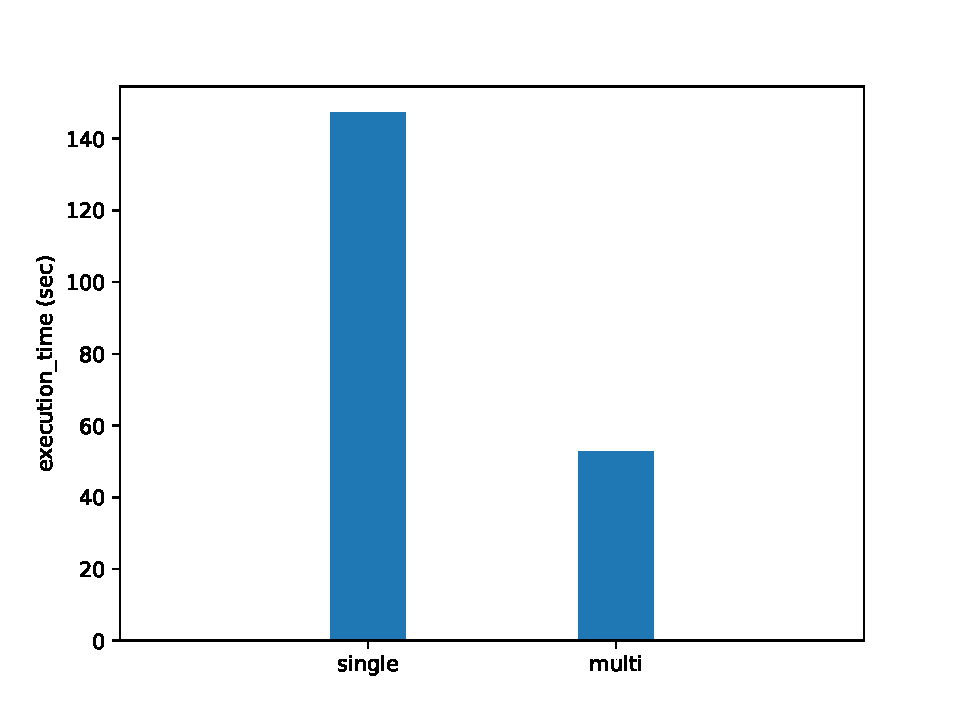
\includegraphics[scale=0.8]{figure/AR_send_num.pdf}
    \caption{Random Walker をまとめて送信したことによる速度向上.}
    \label{Random Walker の送信形態を変化させたときの実行時間}
\end{figure}

\subsection{再利用エッジが貯まるまでに実行する Random Walk の回数}\label{再利用エッジが貯まるまでに実行する Random Walk 実行数}

本実験では, 経路再利用に必要な再利用エッジが貯まるまでに必要な RW 数を測定した. データセットは実世界グラフ, サーバ数は 5 台で実験を行い, RW 実行に関しては終了確率 $\alpha$ = 0.15 の RW を, 各サーバに規定の再利用エッジ数が貯まるまで実行し続けた. 図 \ref{再利用エッジが貯まるまでに実行する Random Walk の回数} に実験結果を示す. 横軸が各サーバに保存された再利用エッジ数, 縦軸が各サーバの RW 実行数の平均を示している. 再利用エッジ数が 6,000,000, 16,000,000, 26,000,000, 36,000,000, 46,000,000 貯まるまでに実行する RW 数はそれぞれ約 1,000,000, 3,130,000, 6,600,000, 12,000,000, 24,000,000 となった. 図 \ref{再利用エッジが貯まるまでに実行する Random Walk の回数} を見てもわかるように, 再利用エッジ数が増えれば増えるほど, さらに再利用エッジを保存するために必要になる RW 実行数が増加する. これは, RWer が同じエッジを何回も通るため新しいエッジを見つけにくくなるからである. 

\begin{figure}[t]
    \centering
    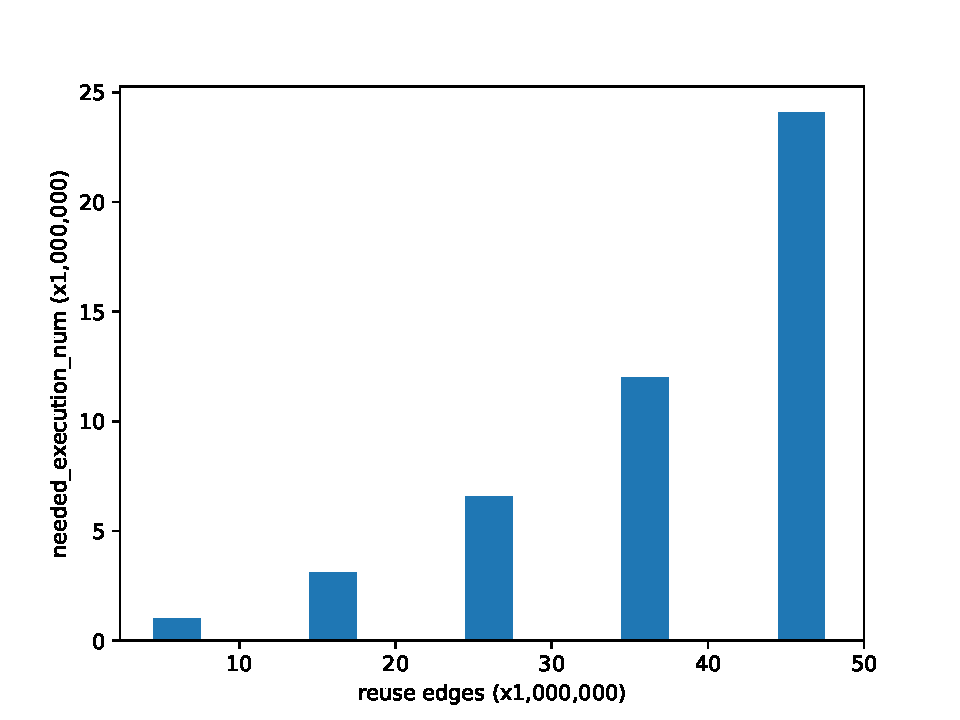
\includegraphics[scale=0.8]{figure/AR_cache_RWer_num.pdf}
    \caption{再利用エッジが貯まるまでに実行する Random Walk の回数.}
    \label{再利用エッジが貯まるまでに実行する Random Walk の回数}
\end{figure}

\chapter{結論}
\label{chap:conclusion}
\section{まとめ}

% 本研究では, 地理的分散環境下に適した RW 実行エンジンを提案した. 提案手法では, 自律的 RW 実行という本手法の用途を意識することに加え, RWer 単位での独立性という RW 演算の特徴に注目し, UDP 通信を使用した非同期処理を採用した. UDP 通信を利用することで, WAN におけるスループットの低下を抑えられる. そして非同期処理を採用することで, 各データセンターによる自律的な RW 実行を実現することができる. また, 提案手法は過去に終了した RWer の経路を再利用することで, RW 遷移時の通信量を削減する機能を有する. 

% 地理的分散環境下を想定した実験の結果, 提案手法は既存手法に比べ $1.6 \sim 7.1$ 倍高速であることがわかった. また提案手法は RTT, パケットロス率が高ければ高いほど, さらにグラフ分割精度が悪ければ悪いほど有効であることがわかった. さらにサーバ数を変化させる実験により, 提案手法が既存手法に比べてシステム規模に対するスケーラビリティに優れていることがわかった. 

本研究では, 地理的分散環境下に適した RW 実行エンジンを提案した. 本研究は, 地理的分散環境下において各データセンターが, 自身が保有する頂点を始点とした RWer の生成・処理を自律的に行い, 結果をそのデータセンターの所在地域が活用することを想定する. この自律的な RW 実行を既存手法の同期処理で実現しようとする場合, 各データセンターにおけるアプリケーション内の RW 実行ごとに全データセンターで同期を行う必要がある. 地理的分散環境下においては, データセンターの増加により同期のための通信が増えることに加え, グラフ分割精度の悪化により同期の回数も増える. そして低帯域・高遅延の通信環境 (WAN) ではこの同期のために何度も発生する通信のオーバヘッドがさらに増加する. 対して提案手法は, 自律的 RW 実行という本手法の用途を意識することに加え, RWer 単位での独立性という RW 演算の特徴に注目し, UDP 通信を使用した非同期処理を採用した. UDP 通信を利用することで, WAN における性能低下を抑えられる. そして非同期処理を採用することで高コストな同期通信を省略し, 各データセンターによる自律的な RW 実行を実現することができる. また, 提案手法は過去に終了した RWer の経路を再利用することで, RW 遷移時の RWer の送信を一部スキップし, 通信量を削減した. 

地理的分散環境を想定した実験の結果, 提案手法は既存手法に比べ 1.6 (経路再利用なし) $\sim$ 7.1 (経路再利用あり) 倍高速であることがわかった. また提案手法は既存手法と異なり RTT, パケットロス率が大きくグラフ分割精度が悪いほど有効であり, サーバ台数を増やした実験で性能が悪化しなかったことからシステム規模に対するスケーラビリティにも優れていることがわかった. 

\section{今後の課題}

\subsection{データセンター内処理を意識したシステム}

提案手法では, 簡単のためデータセンターを一つのサーバとみなして実装を行った. しかし実際はデータセンターは複数のサーバで構成されているため, そのデータセンター内のサーバクラスタでの処理も考える必要がある. 例えば, データセンター内のサーバクラスタでの RW 実行では既存手法のような同期処理を行い, データセンターを一つの塊と見たときの全体としての RW 実行では提案手法のように非同期処理を行うといったアイデアが考えられる. 

\subsection{RWer の経路情報の保存方法}

本研究においては, 終了した RWer を生成サーバに送信して, その生成サーバのみが RWer の経路情報を保存していたが, 他にもいくつか方法が考えられる. 例えば, 終了した RWer を生成サーバだけでなく経由サーバ全てに送信する方法である. これは RWer の経路情報を確認すれば実現可能である. このようにすることで効率的に RWer の経路情報を保存することができる. また, 生存している RWer が他のサーバへ送信されるタイミングでそのサーバに現時点での RWer の経路情報を保存するといった手法も考えられる. 

\bibliographystyle{unsrt}
\bibliography{references}

\chapter*{謝辞}
\label{chap:acknowledgments}
{\small
  \begin{flushright}
    年月日
  \end{flushright}
}
\addcontentsline{toc}{chapter}{謝辞}

% \appendix
% \chapter{タイトル}
% \label{chap:appendix}
% \def\thechapter{\Alph{chapter}}
% \input{appendix}

\end{document}